\begin{SingleSpace}
\chapter{Linking the Climate and Thermal Phase Curve of 55 Cancri e}\label{ch:linking-climate-55cnce}
% \vspace{0.5cm}
% \chapterprecishere{``One face is forever sunlit, and one forever dark, and only the planet's slow liberation gives the twilight zone a semblance of seasons.''\par\raggedleft--- \textup{Stanley G. Weinbaum}, The Lotus Eaters}
\end{SingleSpace}
% \vspace{0.5cm}

\noindent
 \vspace*{-0.5cm}
\textit{Most of the results in this chapter are published in \citet{hammond2017climate}.}
 \vspace*{0.5cm}

% 0 -- LEAD-IN PARAGRAPHS

%START ELEMENT

% Now that I have introduced lava planets and 55 Cancri e in Chapter \ref{ch:lava-planets}, laid out a theory of their circulation in Chapters \ref{ch:wave-mean-flow} and X, and discussed the numerical model I used to simulate them in Chapter \ref{ch:sim-exofms}, I can move to the central question of this thesis. Namely, how to interpret the thermal emission phase curve of a tidally locked lava planet? The remaining chapters of my thesis will investigate this in increasing detail.

%FRAMING TEXT



The first thermal phase curve of a terrestrial exoplanet was measured by \citet{demory201655cnce} using the \textit{Spitzer} space telescope to observe the thermal emission of the ``lava planet'' 55 Cancri e. This followed the measurement of transits in the visible \citep{winn2011super} and infrared
\citep{demory201155cnce}. It was the first observation directly linked to the global circulation of a terrestrial planet outside our solar system, and provides an opportunity to test the theory of atmospheric circulation of terrestrial tidally locked planets that was developed in the previous chapters.

This chapter aims to recreate the observed thermal phase curve of 55 Cancri e with simulations of an idealised atmosphere. I will use the GCM Exo-FMS to model a range of potential atmospheres, with parameters based on analytic predictions of how the phase curve depends on bulk atmospheric properties. The simulations will show that the observed phase curve could be explained by an atmosphere with specific properties. This chapter builds on studies such as \citet{cowan2011statistics}, \citet{menou2012magnetic}, \citet{komacek2016daynightI}, and \citet{zhang2017dynamics}, which all explored the effect of atmospheric properties on the observable global circulation of tidally locked planets.

%SIGNPOSTS

Section \ref{sec:obs-55cnce} gives an overview of observations of 55 Cancri e to date, including the thermal phase curve \citep{demory201655cnce}. Section \ref{sec:scaling-relations} discusses the general circulation of tidally locked planets, and introduces scaling relations from \citet{zhang2017dynamics} that will be used to interpret the phase curve and GCM simulations. Section \ref{sec:sim-lava-planet} discusses the configuration of the simulations of 55 Cancri e in Exo-FMS. Section \ref{sec:results-linking} shows the results of these simulations, focusing on their global temperature distribution and vertical structure. These simulations are post-processed to produce observations in Section \ref{sec:simulated-obs}. Section \ref{sec:discussion} discusses the constraints that this modelling can place on the likely atmospheric composition of this planet.

%SUMMARISE CONCLUSIONS

The model atmosphere that fitted the observations best, ``Test 4'', had a surface pressure of \SI{5}{\bar} and a mean molecular weight of \SI{4.6}{\gram\per\mole}. The phase curve of this test matched the day-side magnitude and phase of the observations, but the simulated night-side thermal emission was too high. Diagnostic estimates of cloud formation suggested that the night-side could be cold enough for SiO clouds to form high on the night-side, reducing the brightness temperature and matching the observations better. The simulations ruled out some atmospheric compositions. An H$_{2}$ atmosphere could not fit the observations as it gave too small a day-night contrast in the simulations and scaling relations. An atmosphere with a very low surface pressure on the order of 1 bar would also not be possible, as it could not reproduce the observed hot-spot shift.

This chapter concludes that an atmosphere could explain the observed phase curve of 55 Cancri e, given a sufficiently high mean molecular weight and high surface pressure. The simulations require a process such as night-side cloud formation to lower the brightness temperature of their night-side, if they are to match the observations. These conclusions highlight the need for further measurements of the atmosphere of 55 Cancri e and other tidally locked planets.

 % This process could be cloud formation from silicates outgassed from the day-side magma ocean.

%


%%%%%%%%%%%%%%%%%%%%%%%%%%%%%%%%%%%%
\newpage
%SECTION 1 -- PHASE CURVE
\section{Observations of 55 Cancri e}\label{sec:obs-55cnce}

This section discusses observations of the planet 55 Cancri e, and considers its possible atmospheric states and composition. I will show the thermal phase curve observed by \citet{demory201655cnce}, and introduce theoretical scaling relations used to interpret the phase curves of tidally locked exoplanets.

%SUBSECTION --
\subsection{55 Cancri e}

55 Cancri e is a ``lava planet'', a rocky super-Earth with radius $1.875\ \mathrm{R_{E}}$ orbiting close to its host star 55 Cancri A \citep{crida201855cnce}. It is expected to be tidally locked due to its proximity to its star \citep{pierrehumbert2018review}, which is supported by the large day-night contrast shown by its thermal phase curve \citep{demory201655cnce}. Transits of 55 Cancri e in the visible \citep{winn2011super} and infrared \citep{demory201155cnce} presented the possibility of characterisation. 55 Cancri e is particularly amenable to observations for a terrestrial planet, owing to its high equilibrium temperature of approximately \SI{2500}{\kelvin} and its large radius \citep{tinetti2016ariel}.


%SUBSECTION --
\subsection{Thermal phase curve}

\begin{figure}
  \centering
    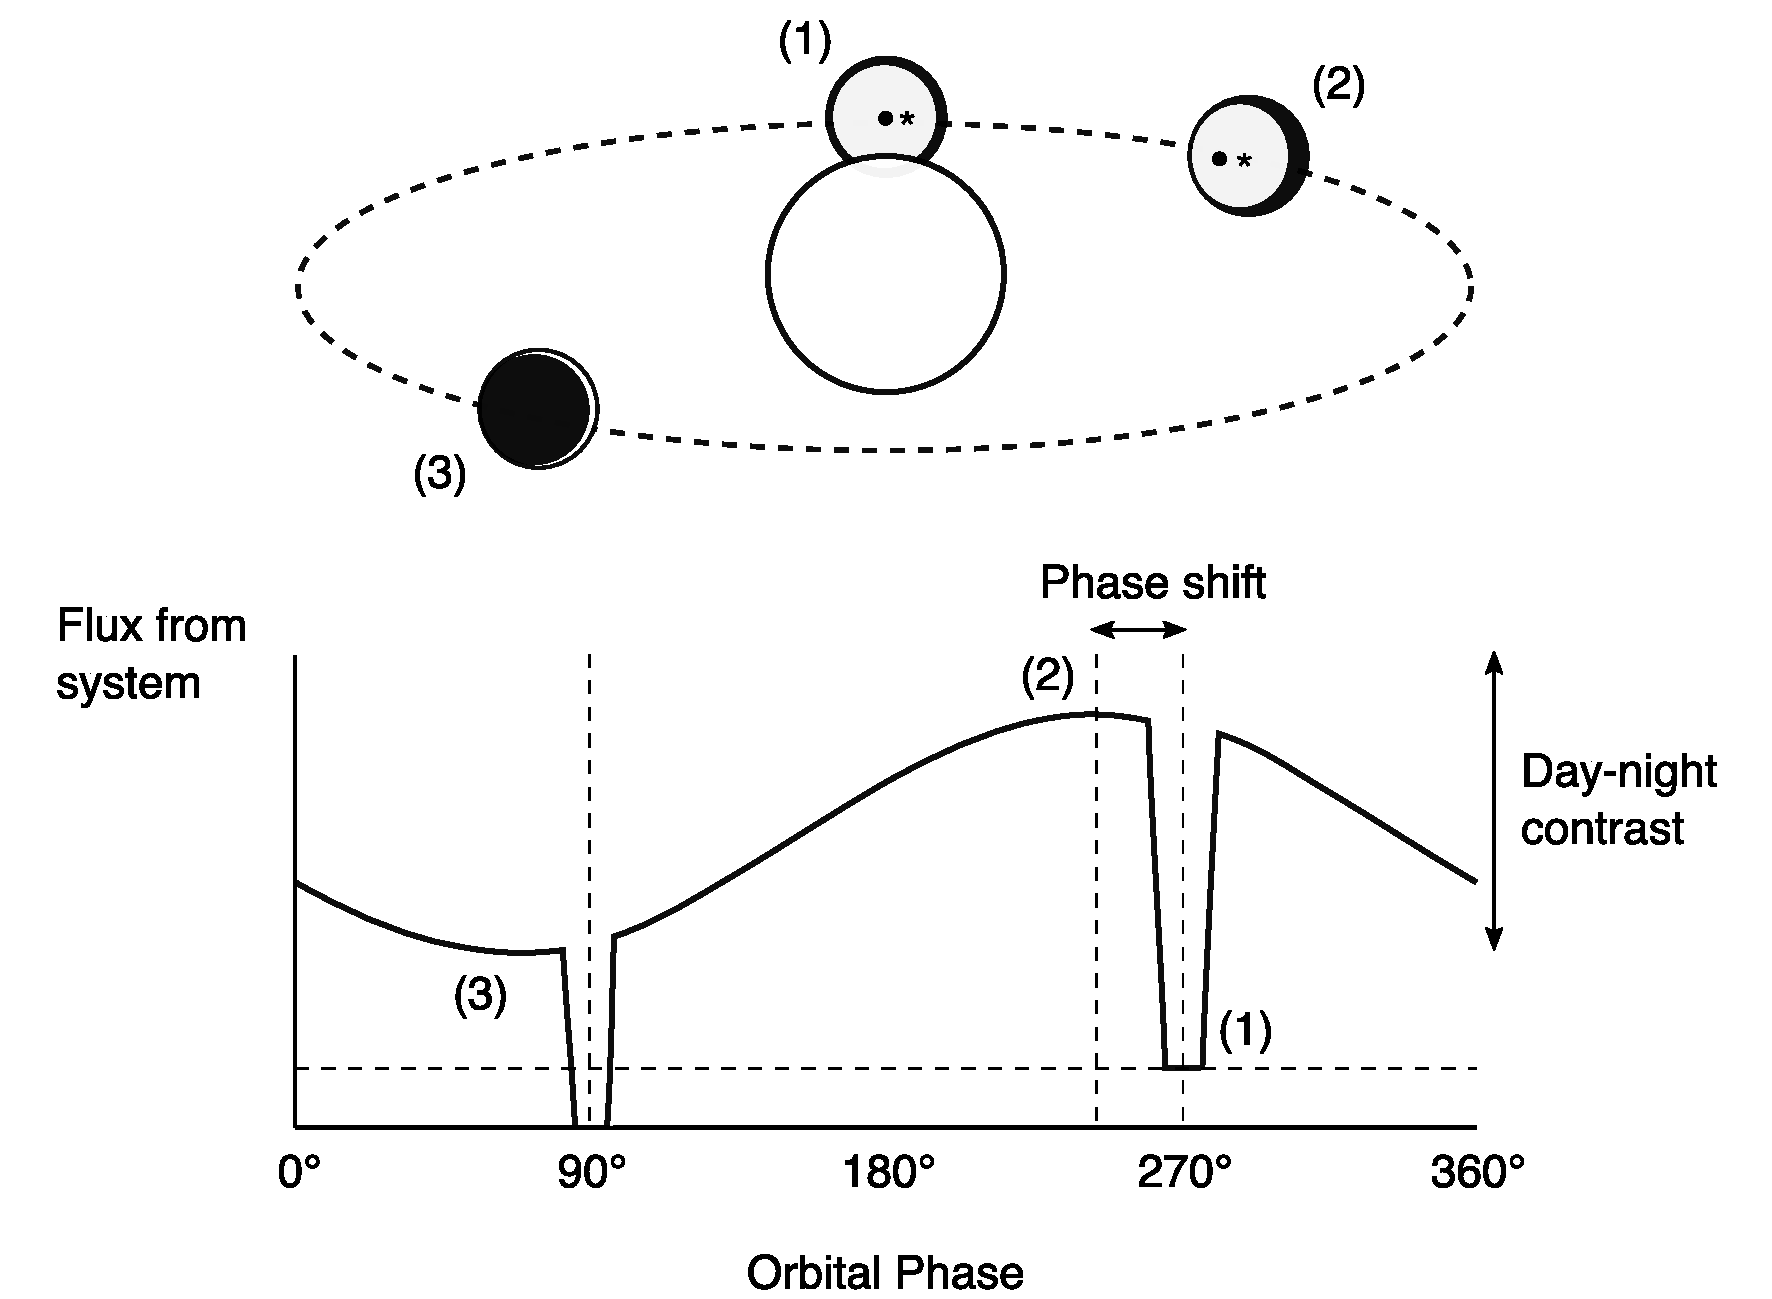
\includegraphics[width=0.9\textwidth]{figures/linking-climate-55cnce/phase-curve-diagram.pdf}
    \caption{A schematic of the phase curve observed of the flux from a planet as it orbits its star. Position 1 is the secondary eclipse, 2 is the phase of the maximum thermal emission, and 3 is the phase of minimum thermal emission.}
    \label{fig:phase-curve-diagram}
\end{figure}

A phase curve is a measurement of the flux from a planet and its star over one orbital period (or averaged over many orbital periods). A ``thermal phase curve'' is the flux at a thermal wavelength, corresponding to the emission of the atmosphere, which is determined by its temperature structure.

Figure \ref{fig:phase-curve-diagram} shows an idealised thermal phase curve of a tidally locked planet, and highlights the key features. At \ang{90}, the planet passes in front of the star, for its transit or ``primary eclipse'', causing a large dip in flux from the system. At \ang{270}, the planet passes behind the star for its ``secondary eclipse'', causing a small dip in flux. The flux above $F/F_{S}=1$ is due to the planet, and is approximately sinusoidal because of the day-side heating and night-side cooling of the planet. The difference in thermal emission between the maximum and minimum of the planet's flux gives the difference in brightness temperature between the day-side and the night-side -- marked on Figure \ref{fig:phase-curve-diagram} as the ``day-night contrast''.

The final key feature is the hot-spot shift, the offset between the peak of the thermal emission and the position of the secondary eclipse. This corresponds to a shift of the hottest part of the planet away from the substellar point. Position 1 in Figure \ref{fig:phase-curve-diagram} is the secondary eclipse, when the observer looks directly at the substellar point (or would, if the star was not in the way). On a bare rock planet, the substellar point (marked by a dot) and the centre of the hottest hemisphere (marked by an asterisk) would coincide, and there would be no phase offset. If a process redistributes heat around the planet, the hottest hemisphere does not have to coincide with the substellar point. Chapter \ref{ch:wave-mean-flow} shows how an atmosphere on a tidally locked planet can have a hot-spot shifted east of the substellar point. Figure \ref{fig:phase-curve-diagram} shows how the observer looks directly at this eastward shifted hot-spot (at position 2) before the secondary eclipse (position 1). So, the maximum flux is measured before the secondary eclipse, and the difference in orbital phase between these two points gives the longitudinal offset between the substellar point and the hottest part of the planet (or just the ``hot-spot'').

Phase curves at optical wavelengths give similar information about the albedo of the planet, showing how features such as clouds affect the reflection of stellar light from the planet at different locations \citep{parmentier2016transitions}. \citet{dragomir2012most} measured an optical phase curve for 55 Cancri e with a similar form to the thermal phase curve in \citet{demory201655cnce}. This raised the possibility that the reflectance and emission are coupled in some way, such as by temperature-dependent clouds.

Figure \ref{fig:demory-phase-curve} shows the thermal phase curve measured by \citet{demory201655cnce} in the \SI{4.5}{\micro\metre} channel of the \textit{Spitzer} telescope \textit{IRAC}\footnote{Infrared Array Camera}. The phase curve has a hot-spot shift of \ang{41}, a day-side temperature of \SI[separate-uncertainty = true]{2700(270)}{\kelvin}, and a night-side temperature of \SI[separate-uncertainty = true]{1380(400)}{\kelvin}. Figure \ref{fig:demory-temp-maps} shows maps of brightness temperature reconstructed from the phase curve. Note that this phase curve is plotted by orbital phase, while the simulated curves later in this chapter are plotted by planetary longitude, meaning that they are reversed along the x-axis.

The combination of this large hot-spot shift and large day-night temperature contrast presents a puzzle. 1D analytic models of circulation on tidally locked planets suggest that a large hot-spot shift implies a strong heat redistribution from day-side to night-side \citep{zhang2017dynamics}. But in the same models, a large day-night contrast implies weak heat redistribution. So, the solutions of \citet{zhang2017dynamics} cannot easily match both of these results.

\citet{angelo201755cnce} reanalysed the phase curve and suggested a hot-spot shift of \ang{34}, a day-side temperature of \SI[separate-uncertainty = true]{2700(160)}{\kelvin}, and a night-side temperature of \SI[separate-uncertainty = true]{1600(140)}{\kelvin}. These are both smaller than the hot-spot shift and day-night contrast reconstructed by \citet{demory201655cnce}, although the two studies are still within error of each other. They are also more consistent with the GCM simulations in this chapter and the predictions of \citet{zhang2017dynamics}, as the smaller hot-spot shift and day-night contrast require a less extreme atmospheric circulation.


\begin{figure}
  \centering
  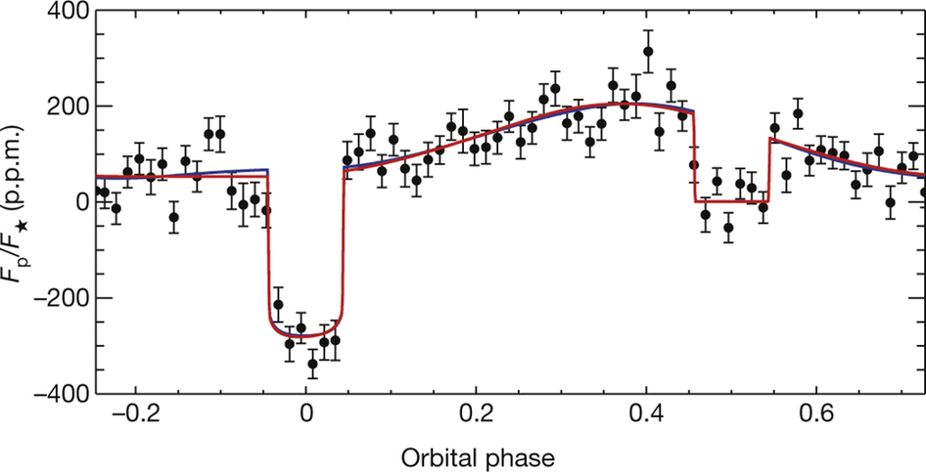
\includegraphics[width=0.7\textwidth]{figures/linking-climate-55cnce/demory-phase-curve.jpg}
\caption{The thermal phase curve observed at \SI{4.5}{\micro\metre} by \citet{demory201655cnce}, showing an offset of the maximum flux from the secondary eclipse, corresponding to a hot-spot shift. Reproduced from \citet{demory201655cnce} with permission.}\label{fig:demory-phase-curve}
\end{figure}

\begin{figure}
  \centering
  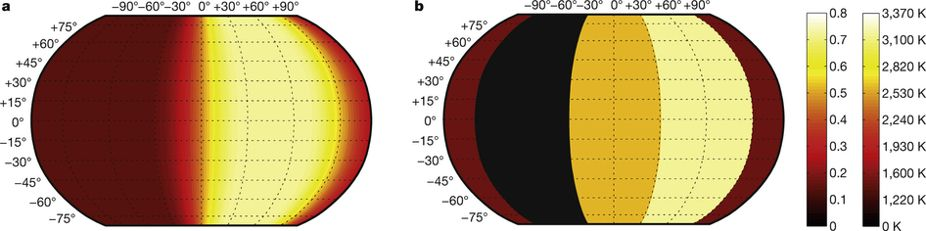
\includegraphics[width=0.95\textwidth]{figures/linking-climate-55cnce/demory-temp-maps.jpg}
\caption{The temperature map reconstructed by \citet{demory201655cnce} from the phase curve in Figure \ref{fig:demory-phase-curve}, showing a hot-spot shift of \ang{41}, a day-side temperature of \SI[separate-uncertainty = true]{2700(270)}{\kelvin}, and a night-side temperature of \SI[separate-uncertainty = true]{1380(400)}{\kelvin}. Reproduced from \citet{demory201655cnce} with permission.}\label{fig:demory-temp-maps}
\end{figure}

%SUBSECTION --
\subsection{Atmospheric Composition}

It is not clear what sort of atmosphere, if any, to expect on a planet like 55 Cancri e. An atmosphere like a hot Jupiter with a low molecular weight seems unlikely, given the planet's proximity to its star and correspondingly high temperatures and high-energy radiation, which would cause atmospheric escape of lighter components \citep{demory201655cnce}. \citet{gillon2012improved} used the observational mass and radius to suggest that there is an atmosphere composed of high molecular weight volatiles.

\citet{tsiaras2016detection} reported the detection of an atmosphere due to spectroscopic deviations from a bare-rock planet, using observations in the near-infrared with the WFC3 camera of the Hubble Space Telescope (HST). In this chapter, I avoid direct questions of atmospheric composition or origin, focusing on what bulk properties -- surface pressure, mean molecular weight, and longwave optical thickness -- could be consistent with the observed thermal phase curve.
%
% %SUBSECTION --
% \subsection*{Atmospheric Circulation}
%
% This chapter simulates possible atmospheres on 55 Cancri e to test if the features of the observed thermal phase curve -- particularly the hot-spot shift and day-night contrast -- are consistent with an atmosphere circulating heat around the planet. Previous similar studies have simulated hot Jupiters and compared their phase curve to observations \citep{showman2015circulation} \citep{mayne2017hotjupiter}. These simulations have proved very useful in understanding their global circulation and behaviour at different temperatures, so it is a natural next step to apply them to observations of a terrestrial planet.
%
% \citet{zhang2017dynamics} suggested scaling relations to predict how the observable hot-spot shift and day-night contrast depend on the properties of the atmosphere of a tidally locked planet. I will use these to predict a likely parameter space that could fit the observations, and to analyse the GCM simulations. Chapter \ref{ch:wave-mean-flow} showed how some of the scaling relations are identical to the shallow-water scaling relations derived in that chapter for the equator of a tidally locked planet. \citet{komacek2016daynightI} tested similar scaling relations against a suite of simulations of hot Jupiters, and found the predictions to be consistent with the behaviour of the GCM. This supports the use of similar scaling relations to interpret the global circulation of the similar tidally locked planet 55 Cancri e.

%SECTION CONCLUSIONS

% Aim of this chapter is to test whether the thermal phase curve is consistent with an atmosphere, and if so what it suggests about the atmosphere.




%%%%%%%%%%%%%%%%%%%%%%%%%%%%%%%%%%%%
%SECTION 2 -- SCALING
\section{Simplified Scaling Theory}\label{sec:scaling-relations}

The section applies scaling relations from the idealised 1D atmospheric models of \citet{zhang2017dynamics} to understand how the atmospheric properties affect the observed phase curve. The relations predict the effect of the bulk properties of the atmosphere on the main features of the phase curve -- the hot-spot shift and day-night contrast. I will describe these scaling relations and show how they were used to select a parameter space of atmospheres that could fit the observed phase curve.

%SUBSECTION --
\subsection{1D Circulation Model}\label{sec:zhang-model}

\citet{zhang2017dynamics} model the circulation on a tidally locked planet with a 1D differential equation on the equator where heat transport is determined by a balance of the radiative timescale and advective timescale \citep{komacek2016daynightI}. The resulting scaling relations are similar to those derived from the shallow-water system in Chapter \ref{ch:wave-mean-flow}. The important timescales in these relations are the radiative timescale $\tau_{\mathrm{rad}}$, the wave timescale $\tau_{\text { wave }}$, and the advective timescale $\tau_{\mathrm{adv}}$. The radiative timescale is the typical timescale of changes due to radiative forcing:

\begin{equation}
  \tau_{\mathrm{rad}} \sim \frac{p_{\tau=1}}{\mu g} \frac{c_{p}}{4 \sigma T^{3}},
\end{equation}

where $p_{\tau=1}$ is the pressure at which the optical thickness is unity, $\mu$ is the mean molecular weight, $T$ is the equilibrium temperature of the planet, and $c_{p}$ is the atmospheric molar heat capacity. The wave timescale is the time for planetary-scale equatorial waves to propagate horizontally:

\begin{equation}
  \tau_{\text { wave }}=L / N H,
\end{equation}

where $L$ is the radius of the planet, $N$ is the buoyancy frequency of the atmosphere, and $H$ is the atmospheric scale height. The advective timescale is the time for the mean zonal flow (the equatorial jet) to advect air around the planet:

\begin{equation}
  \tau_{\mathrm{adv}}=L / U_{\mathrm{eq}}.
\end{equation}

Here, $U_{\mathrm{eq}}$ is the ``wind speed that would result
from acceleration of the wind from day to night due to the day-night pressure gradient if the day-night temperature difference
were in radiative equilibrium and if the Rossby number exceeds
unity'' \citep{zhang2017dynamics}:

\begin{equation}
  U_{\mathrm{eq}}=\left(R \Delta T_{\mathrm{eq}} \Delta \ln p / 2 \mu\right)^{1 / 2},
\end{equation}

where $\Delta T_{\mathrm{eq}}$ is the day-night temperature difference, and ``$ \Delta \ln p$ is the difference in log
pressure between some deep pressure where the day-night
temperature difference is small (10 bars in the theory and
simulations from \citet{komacek2016daynightI}) and some
smaller pressure of interest in the observable atmosphere'' \citep{zhang2017dynamics}.

%The usefulness of this simple model led to the work in Chapters \ref{ch:eqm-zonal-flow} and \ref{ch:wave-mean-flow}, to predict the jet speed and global temperature distribution using a linear shallow-water model.


%SUBSECTION --
\subsection{Hot-Spot Shift}\label{sec:hot-spot-shift}

The hot-spot shift is an observable consequence of the atmospheric circulation on a tidally locked planet. \citet{zhang2017dynamics} predict the longitude of the maximum temperature $\lambda_{m}$ (i.e. the hot-spot shift) to be given by:

\begin{equation}\label{eqn:zhang-hss}
  \sin \left(\lambda_{s}-\lambda_{m}\right) e^{\lambda_{m} / \xi}=\frac{\eta}{\xi \cos \lambda_{s}},
\end{equation}

where

\begin{equation}
  \eta=\frac{\xi}{1+\xi^{2}} \frac{e^{\frac{\pi}{2 \xi}}+e^{\frac{3 \pi}{2 \xi}}}{e^{\frac{2 \pi}{\xi}}-1},
\end{equation}

for $\xi=\tau_{\mathrm{rad}} / \tau_{\mathrm{adv}}$ and $\lambda_{s}=\tan ^{-1} \xi$. When $\lambda_{m}$ is small in this expression, $\lambda_{m} \approx \lambda_{s}$ and it reduces to the same expression as in Chapter \ref{ch:wave-mean-flow}, $\lambda_{m}=\tan ^{-1} (\tau_{\mathrm{rad}} / \tau_{\mathrm{adv}})$. This expression assumes that the hot-spot shift depends on a balance of eastward heat transport versus radiation to space. It does not represent the effect of the stationary waves that are so important to the global temperature distribution, so does not apply in regimes where these dominate or in regions away from the equator \citep{perez2013atmospheric, hammond2018wavemean}.

%SUBSECTION --
\subsection{Day-Night Contrast}\label{sec:day-night-contrast}

The day-night contrast on a tidally locked planet refers to the fractional difference between the temperature difference between the day-side and the night-side, compared to the temperature difference that would be expected in radiative equilibrium.

\citet{zhang2017dynamics} use the 1D model to predict the day-night contrast to be:

\begin{equation}\label{eqn:zhang-dnc}
  A=\frac{\Delta T}{\Delta T_{\mathrm{eq}}} \sim 1-\frac{2}{\alpha+\sqrt{\alpha^{2}+4 \gamma^{2}}}
\end{equation}

where the non-dimensional parameters $\alpha$ and $\gamma$ are

\begin{equation}
  \begin{gathered}
\alpha=1+\frac{\left(\Omega+\frac{1}{\tau_{\text { drag }}}\right) \tau_{\text { wave }}^{2}}{\tau_{\text { rad }} \Delta \ln p} \\
\gamma=\frac{\tau_{\text { wave }}^{2}}{\tau_{\text { rad }} \tau_{\text { adv }, \text { eq }} \Delta \ln p}
\end{gathered}
\end{equation}

A short radiative timescale $\tau_{\text { rad }}$ gives a large day-night contrast $A$. This is because the heated air on the day-side radiates away its energy faster than it can be transported to the night-side by jet advection or wave transport \citep{zhang2017dynamics, hammond2017climate}. From the alternative point of view of a global circulation governed by stationary waves, this is because the high radiative damping rate brings the forced wave response into phase with the forcing and strengthens it, as discussed in Chapter \ref{ch:wave-mean-flow} \citep{hammond2018wavemean}. Section \ref{sec:discussion} compares these mechanisms in more detail.

% It is not clear whether these are two different views of the same process, or really are two different processes. It may be that the first description does not properly capture the effect of wave dynamics and the second picture does not represent the effect of advection. In reality, the different mechanisms may be more appropriate for different types of planet.


%SUBSECTION --
\subsection{Parameter Space of Simulations}\label{sec:param-space}

Figure \ref{fig:param_map} shows a parameter space in atmospheric surface pressure and mean molecular weight, predicted by the 1D scaling relations to be potentially consistent with the observed thermal phase curve. The red line shows the region in which Equation \ref{eqn:zhang-hss} predicts the hot-spot shift is greater than \ang{20}. The blue line shows the region in which the day-night contrast is predicted to be greater than 80\% by Equation \ref{eqn:zhang-dnc}. The region shaded in green between these lines shows the parameter space that could support both a significant hot-spot shift and day-night contrast. The next section uses this parameter space to select a suite of GCM simulations to compare to the observed phase curve.

\begin{figure}
  \centering
  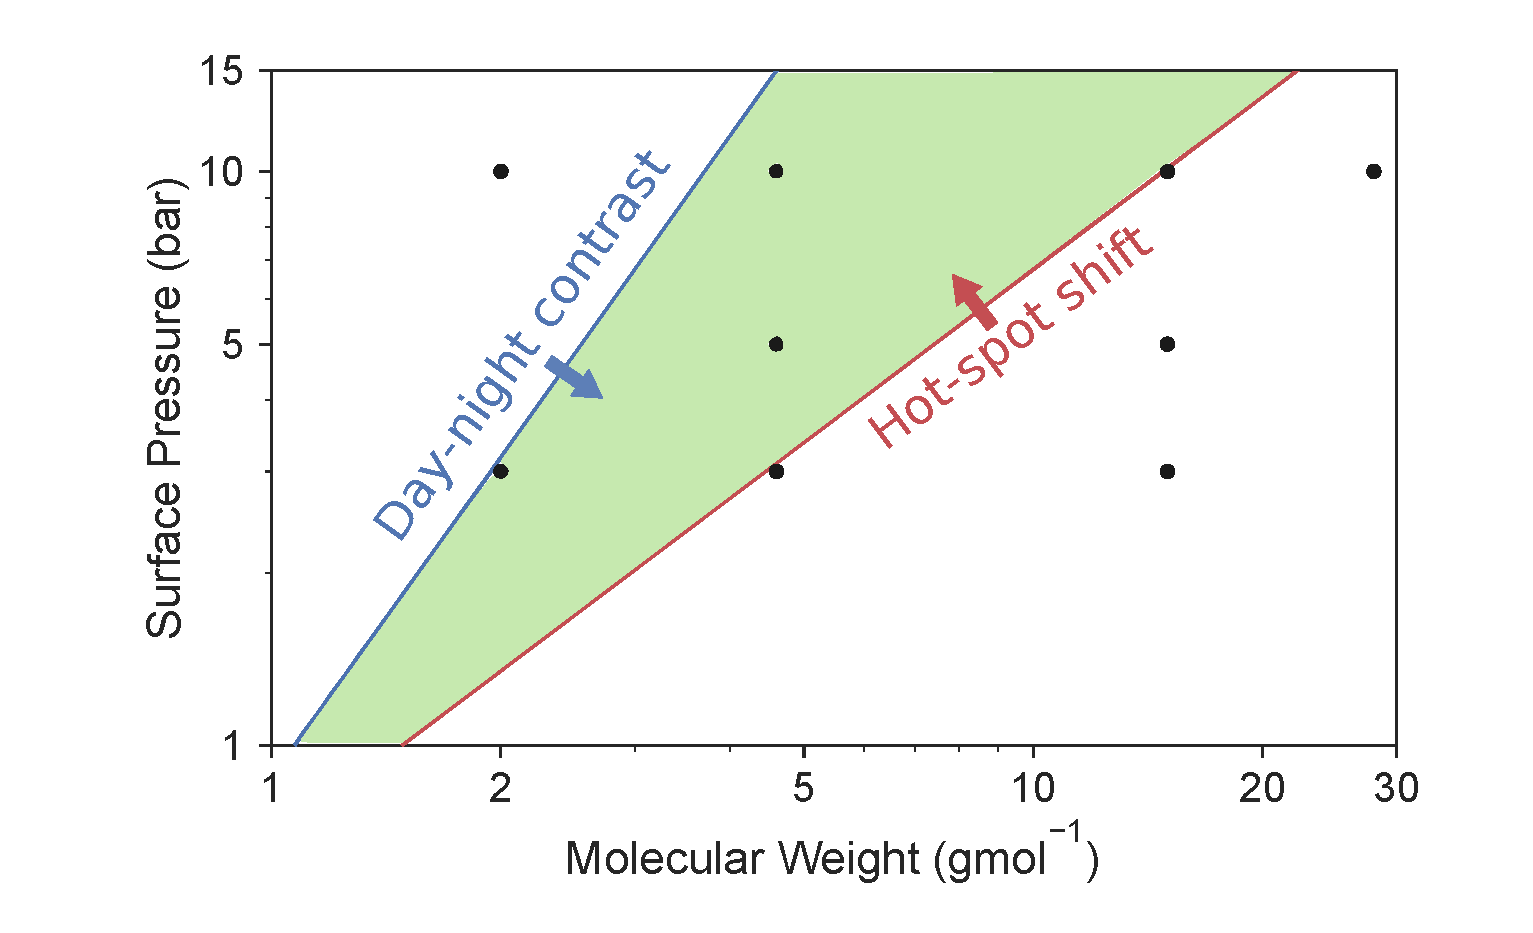
\includegraphics[width=0.75\textwidth]{figures/linking-climate-55cnce/param_map_edited.eps}
\caption{The atmospheric parameter space under consideration, where the green region is predicted by the relations of \citet{zhang2017dynamics} to support both a significant hot-spot shift and day-night contrast. The black points show the parameters of the GCM tests. The hot-spot shift and day-night contrast were calculated with a bulk wind speed of \SI{1000}{\metre\per\second} and a mean temperature \SI{2000}{\kelvin}. The two lines correspond to a hot-spot shift of \ang{20} and a day-night contrast of 80\%.}\label{fig:param_map}
\end{figure}

%SECTION CONCLUSIONS

%%% UP TO HERE


%%%%%%%%%%%%%%%%%%%%%%%%%%%%%%%%%%%%
%SECTION 3 -- SIMULATIONS
\section{Exo-FMS Configuration}\label{sec:sim-lava-planet}

This section describes how the GCM Exo-FMS was configured to simulate a suite of idealised atmospheres on 55 Cancri e. The parameters of the simulations were selected using the scaling relations discussed above, to investigate the atmospheric parameter space that could be consistent with the observations.

% %SUBSECTION --
% \subsection{Exo-FMS Setup}\label{sec:exofms-setup}

Appendix \ref{ap:exo-fms} describes the structure and components of Exo-FMS in detail. It is based on the Flexible Modelling System structure and associated latitude-longitude dynamical core from the Geophysical Fluid Dynamics Laboratory (GFDL). Similar models based on the FMS structure have been used to investigate other terrestrial and tidally locked planets \citep{merlis2010atmospheric, heng2011atmospheric, koll2015phasecurves, koll2016temperature}. The general results of simulations of these tidally locked planets are not sensitive to the choice of model, as shown by the similar results of studies using different 3D atmospheric models \citep{carone2014connecting, kataria2014atmospheric, charnay20153d}.

The simulations were all configured with a radius $r_{p} = 1.91\ R_{Earth}$, orbital period $P = 0.737\ \mathrm{days}$, surface gravity $g =$ \SI{21.7}{\metre\per\second\squared} \citep{demory201655cnce}, incoming stellar flux \SI[scientific-notation=true]{3.55e6}{\watt\per\metre\squared} \citep{von201155}, and zero surface and atmospheric albedo. The model itself used a 144 by 96 by 40 grid, with vertical levels set by a hybrid sigma-pressure system, where the top pressure level was approximately $10^{-5}p_{s}$ for surface pressure p\textsubscript{s}. A dry convective adjustment scheme was applied to every column, with instantaneous adjustment to a dry adiabat where the profile was convectively unstable. The radiative transfer was modelled with a two-stream semi-grey scheme with variable longwave optical depth that scaled linearly with pressure, and zero shortwave optical depth. The default longwave optical depth of 10 was chosen to approximate the observed day-side temperature.

This optical depth was also consistent with the surface temperature achieved by a 10 bar $\mathrm{H_2}$ atmosphere, using a one-dimensional radiative-convective model with two-stream radiative transfer calculated using the $\mathrm{H_2}$ collisional opacity \citep{pierrehumbert2011hydrogen}. This corresponds to an opacity $\kappa$ of \SI{22.4}{\cm\squared\per\kg}, which I used in all the tests apart from those where the opacity was explicitly varied. In reality, $\kappa$ could be different, and would not scale linearly with pressure -- a more realistic representation such as that in Chapter \ref{ch:clouds-lava-planets} would be needed to interpret future observations.

The simulations were initialised from rest with every atmospheric column on a dry adiabat from a specified surface temperature, up to a given pressure level where the profile was set to an isothermal stratosphere. The simulation results were not sensitive to the initial conditions, owing to the short radiative timescale of the atmosphere. The atmosphere reached radiative equilibrium when the outgoing longwave radiation and top-of-atmosphere temperatures stopped evolving. Dynamical equilibrium was reached when the maximum zonal winds and total angular momentum stabilised. All the results presented are averaged over the final 10 days of simulation runs of at least 50 Earth days, after the model reached equilibrium.


% %SUBSECTION --
% \subsection{Suite of Tests}\label{sec:test-suite}

The suite of GCM tests listed in Table \ref{tab:gcm-test-suite} were chosen to cover the region that Figure \ref{fig:param_map} predicted to fit the observations, according to the scaling relations in Section \ref{sec:scaling-relations},. Some simulations test the effect of a particular parameter in more detail, such as Tests 3, 4, and 5, which test the effect of changing the surface pressure $p_{s}$. The next section will discuss the simulations and show the effect of the surface pressure, mean molecular weight, and longwave optical depth on the global circulation and thermal phase curve.


\begin{table}[]
\begin{tabular}{l|llll|ll}
\textbf{Test} & \textbf{Composition} & $p_{s}$ & $\mu$  & $\tau_{\infty}$ & \textbf{Hot-Spot Shift} & \textbf{Day-Night Contrast} \\
\hline
 1    & H\textsubscript{2}  & 10   & 2.0  & 8 & \SI[retain-explicit-plus]{+45}{\degree} & \SI{100}{\kelvin}  \\
 2    & N\textsubscript{2}  & 10   & 28.0  & 8 & \ang{0} & \SI{750}{\kelvin}  \\
 3    & H\textsubscript{2} + N\textsubscript{2}  & 10   & 4.6  & 8 &  \SI[retain-explicit-plus]{+30}{\degree} & \SI{200}{\kelvin}  \\
 4    & H\textsubscript{2} + N\textsubscript{2}  & 5   & 4.6  & 8 &  \SI[retain-explicit-plus]{+25}{\degree} & \SI{250}{\kelvin}  \\
 5    & H\textsubscript{2} + N\textsubscript{2}  & 3   & 4.6  & 8 &  \SI[retain-explicit-plus]{+15}{\degree} & \SI{300}{\kelvin}  \\
 6    & H\textsubscript{2} + N\textsubscript{2}  & 10   & 15.0 & 8 & \ang{0}& \SI{1500}{\kelvin}  \\
 7    & H\textsubscript{2} + N\textsubscript{2}  & 5   & 15.0  & 8 & \ang{0}& \SI{550}{\kelvin}  \\
 8    & H\textsubscript{2} + N\textsubscript{2}  & 3   & 15.0  & 8 & \ang{0}& \SI{600}{\kelvin}  \\
 9    & H\textsubscript{2} + N\textsubscript{2}  & 5   & 14.6  & 2 &  \SI[retain-explicit-plus]{+20}{\degree} & \SI{200}{\kelvin}  \\
 10    & H\textsubscript{2} + N\textsubscript{2}  & 5   & 4.6  & 4 &  \SI[retain-explicit-plus]{+20}{\degree} & \SI{250}{\kelvin}  \\
11    & H\textsubscript{2} + N\textsubscript{2}  & 5   & 4.6  & 8 &  \SI[retain-explicit-plus]{+25}{\degree} & \SI{250}{\kelvin}
\end{tabular}
\caption{The suite of GCM simulations, testing the effect of varying the atmospheric mean molecular weight $\mu$, surface pressure $p_{s}$, and optical thickness $\tau_{\infty}$. The hot-spot shifts are rounded to the nearest \ang{5}, and the day-night contrasts to the nearest \SI{50}{\kelvin}. The observed phase curve has a hot-spot shift of \SI[separate-uncertainty = true,retain-explicit-plus]{+41(12)}{}$^\circ$ and a day-night contrast of \SI[separate-uncertainty = true]{1300(670)}{\kelvin}. Test 4 is the ``best-fit'' test discussed in Section \ref{sec:discussion}.}\label{tab:gcm-test-suite}
\end{table}


%SECTION CONCLUSIONS



%%%%%%%%%%%%%%%%%%%%%%%%%%%%%%%%%%%%
%SECTION 4 -- RESULTS
\section{Simulation Results}\label{sec:results-linking}

This section discusses the results of the simulations in Exo-FMS. I will show the effect of varying the mean molecular weight, surface pressure, and optical thickness of the atmosphere, and compare the results to the theory in Section \ref{sec:scaling-relations}. The simulations generally follow the scaling relations discussed above, but none of them exactly match the temperature distribution inferred from the observed phase curve.

%SUBSECTION --
\subsection{Effect of Mean Molecular Weight}\label{sec:mmw_effect}

The first set of tests investigate the effect of the mean molecular weight $\mu$ on the global circulation and thermal phase curve. I selected a range of molecular weights from \SI{2.0}{\gram\per\mol} (H\textsubscript{2}) to \SI{28.0}{\gram\per\mol} (N\textsubscript{2}) from the parameter space in Section \ref{sec:param-space}.

Test 1 is a pure H\textsubscript{2} atmosphere with $\mu =$ \SI{2.0}{\gram\per\mol}, surface pressure $p_{s} = 10\ \mathrm{bar}$ and optical thickness $\tau_{\infty}= 8.0$. Section \ref{sec:scaling-relations} predicts that this atmosphere will have a large hot-spot shift but a small day-night contrast, due to its high specific heat capacity, giving a long radiative timescale. Figure \ref{fig:Tlevels-maps} confirms this prediction, showing that it has a large hot-spot shift in the second plot showing the mid-atmosphere, with the hottest hemisphere centred at about \ang{45}. \citet{kataria2014atmospheric} also showed that a lower molecular weight atmosphere had a larger hot-spot shift in simulations of the atmosphere of a super-Earth. Figure \ref{fig:Tlevels-maps} also shows that the day-night contrast is small, because of the highly efficient heat redistribution. The surface air temperature in the first plot does not show such a large hot-spot shift, as it is closely coupled to the incoming stellar flux. The third plot shows the brightness temperature, which is calculated directly from the outgoing longwave radiation of the semi-grey radiative transfer scheme. This corresponds to a very low pressure due to the high longwave optical depth of the atmosphere, meaning that the brightness temperature is almost homogeneous as it probes the upper atmosphere where the heat circulation is very efficient.

Test 2 is a pure N\textsubscript{2} atmosphere with $\mu =$ \SI{28.0}{\gram\per\mol}, surface pressure $p_{s} = 10\ \mathrm{bar}$ and optical thickness $\tau_{\infty}= 8.0$. Section \ref{sec:scaling-relations} predicts that this atmosphere will have a large day-night contrast but a small hot-spot shift, due to its low specific heat capacity, giving a short radiative timescale. Figures \ref{fig:Tlevels-maps} and \ref{fig:pressure_variation} confirm this prediction, showing a large difference in day-side and night-side temperature at all pressure levels, and in the brightness temperature. The hot-spot is centred on the substellar point, also confirming the prediction of a small or zero hot-spot shift.

These two extremes of $\mu$ behave as predicted by Section \ref{sec:scaling-relations}, suggesting that an intermediate value of $\mu$ may fit the observations better. Test 3 is a mixture of H\textsubscript{2} and N\textsubscript{2}, with $\mu =$ \SI{4.6}{\gram\per\mole}, surface pressure $p_{s} = 10\ \mathrm{bar}$ and optical thickness $\tau_{\infty}= 8.0$. Figure \ref{fig:Tlevels-maps} shows that at the half-surface-pressure level, and in the brightness temperature, there is a significant hot-spot shift and day-night contrast (although not as large as that observed by \citet{demory201655cnce}). I will simulate the thermal phase curves of these tests later for a more direct comparison to the observations.

The rest of this chapter will show the effect of the surface pressure and longwave optical thickness on the global circulation and simulated phase curve. Of these first three tests, Tests 1 and 2 reproduce the observed hot-spot shift or day-night contrast respectively -- but not both. Test 3 has a significant hot-spot shift and day-night contrast, but neither is as large as the observations. All these tests qualitatively match the predictions of the scaling relations in Section \ref{sec:scaling-relations}.

\begin{figure}
  \begin{subfigure}[t]{0.32\textwidth}
    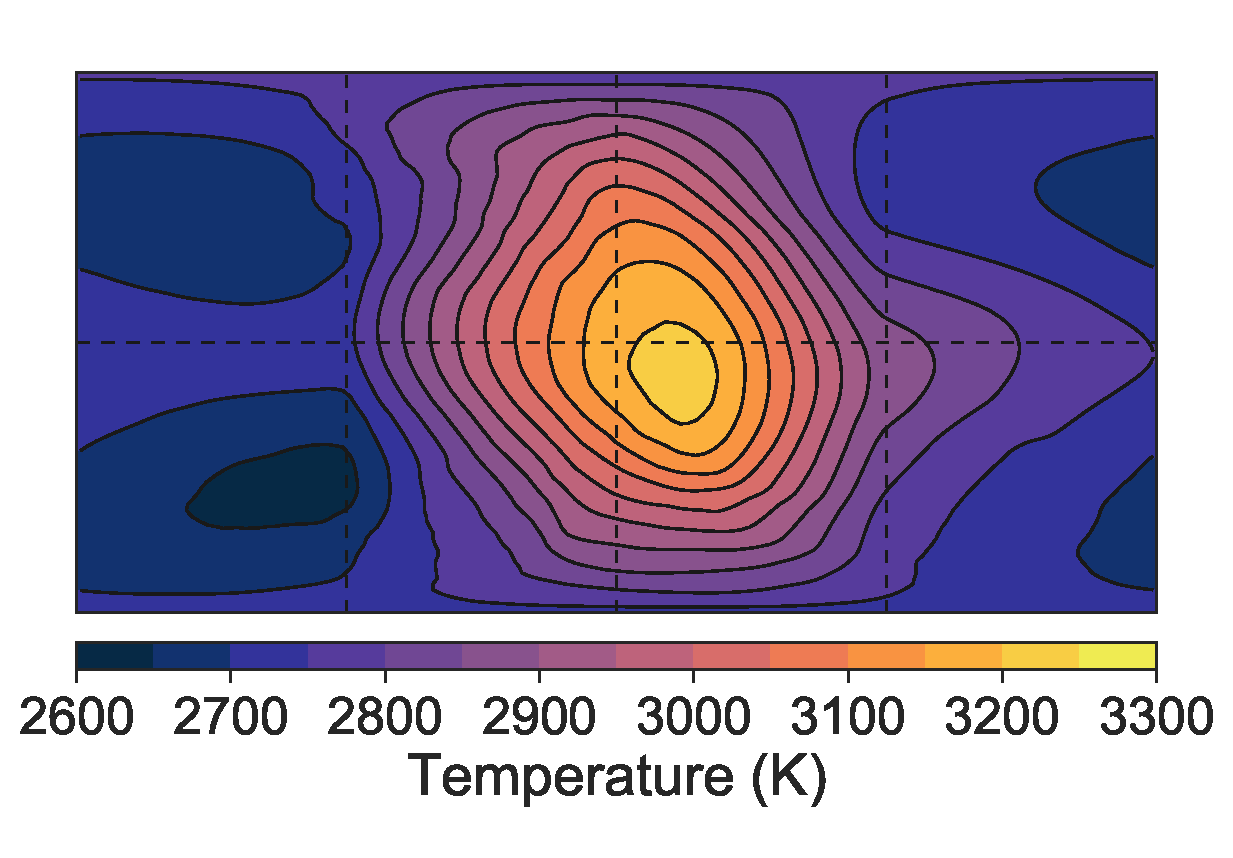
\includegraphics[width=\textwidth]{figures/linking-climate-55cnce/H210bar_surfp.eps}
    \caption{Test 1 surface.}
    \label{fig:free-u-shear}
  \end{subfigure}
\enskip
  \begin{subfigure}[t]{0.32\textwidth}
    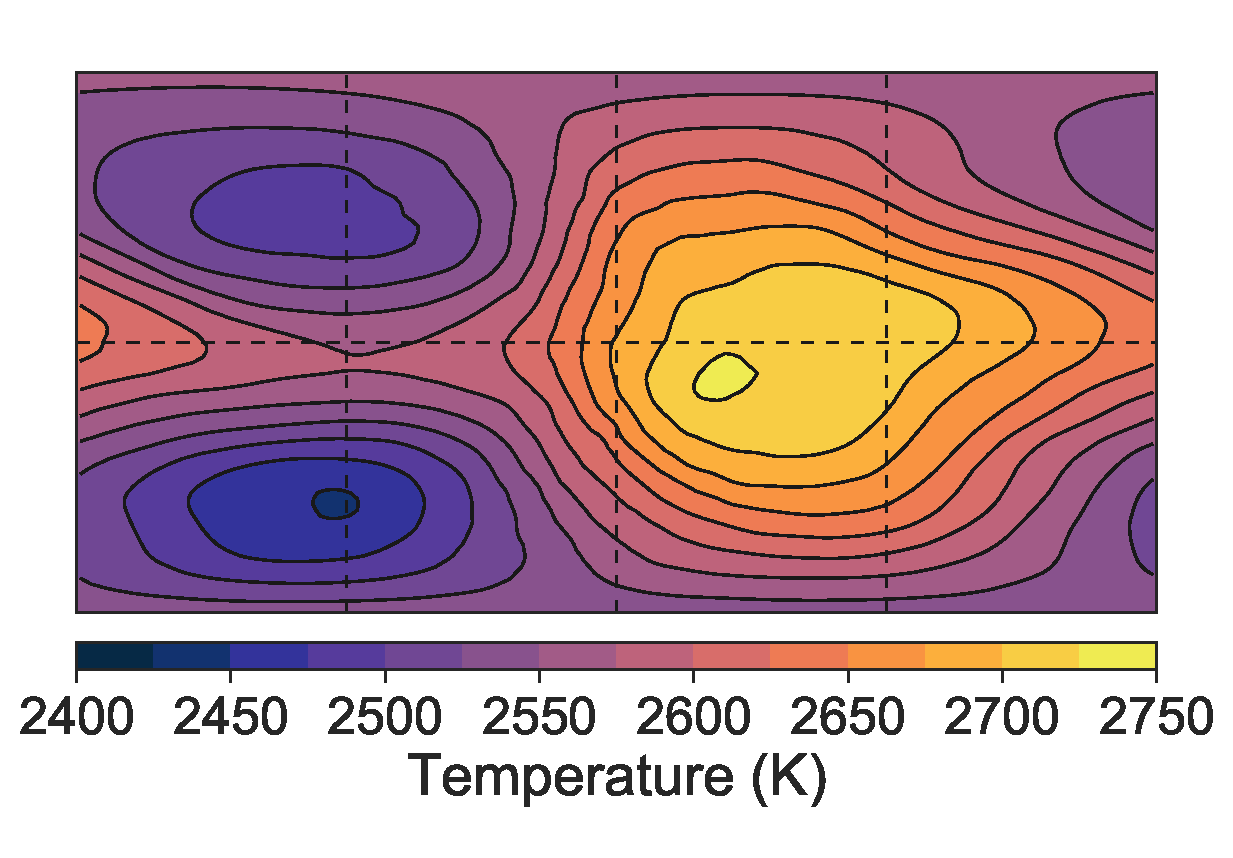
\includegraphics[width=\textwidth]{figures/linking-climate-55cnce/H210bar_halfp.eps}
    \caption{Test 1 mid-atmosphere.}
    \label{fig:free-v-shear}
  \end{subfigure}
\enskip
  \begin{subfigure}[t]{0.32\textwidth}
    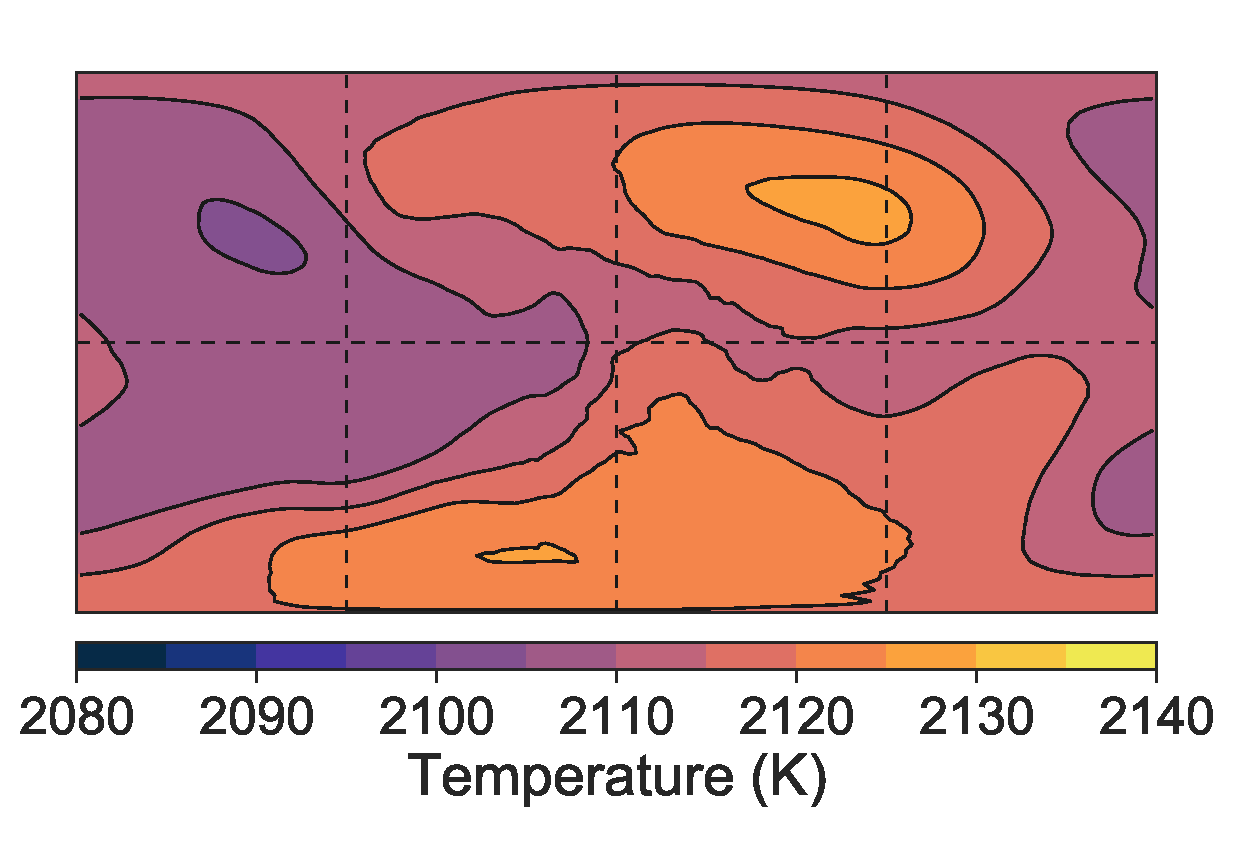
\includegraphics[width=\textwidth]{figures/linking-climate-55cnce/H210bar_brightT.eps}
    \caption{Test 1 brightness.}
    \label{fig:free-h-shear}
  \end{subfigure}
  \\
  \begin{subfigure}[t]{0.32\textwidth}
    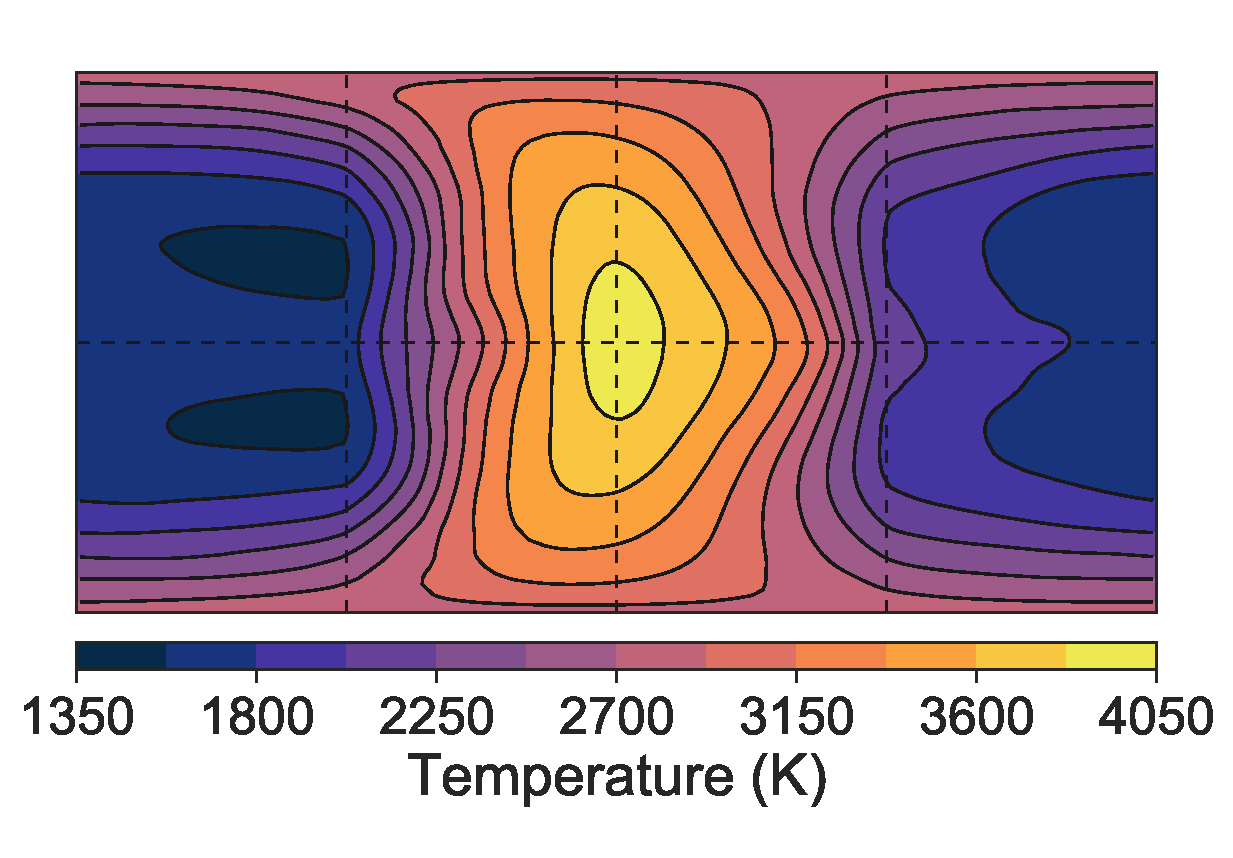
\includegraphics[width=\textwidth]{figures/linking-climate-55cnce/N2_surfp.eps}
    \caption{Test 2 surface.}
    \label{fig:free-u-shear}
  \end{subfigure}
\enskip
  \begin{subfigure}[t]{0.32\textwidth}
    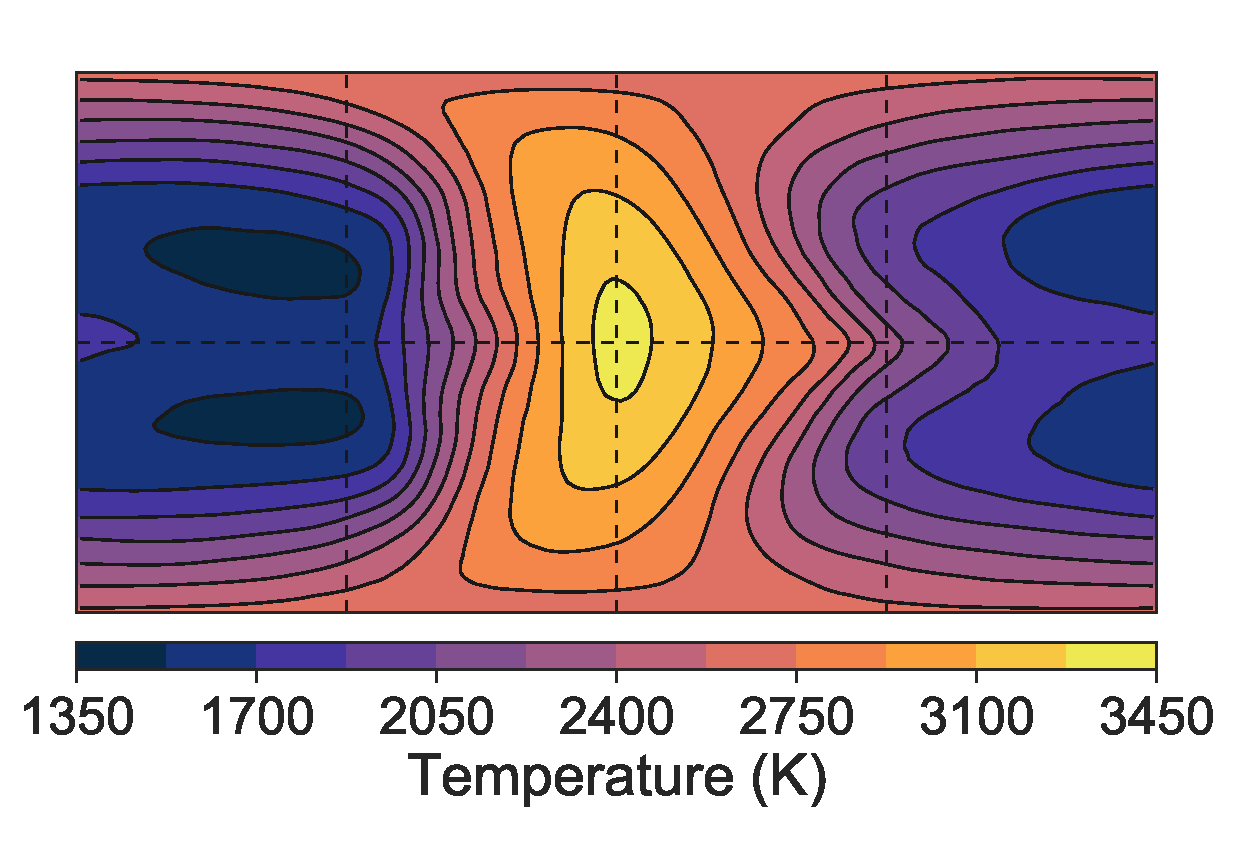
\includegraphics[width=\textwidth]{figures/linking-climate-55cnce/N2_halfp.eps}
    \caption{Test 2 mid-atmosphere.}
    \label{fig:free-v-shear}
  \end{subfigure}
\enskip
  \begin{subfigure}[t]{0.32\textwidth}
    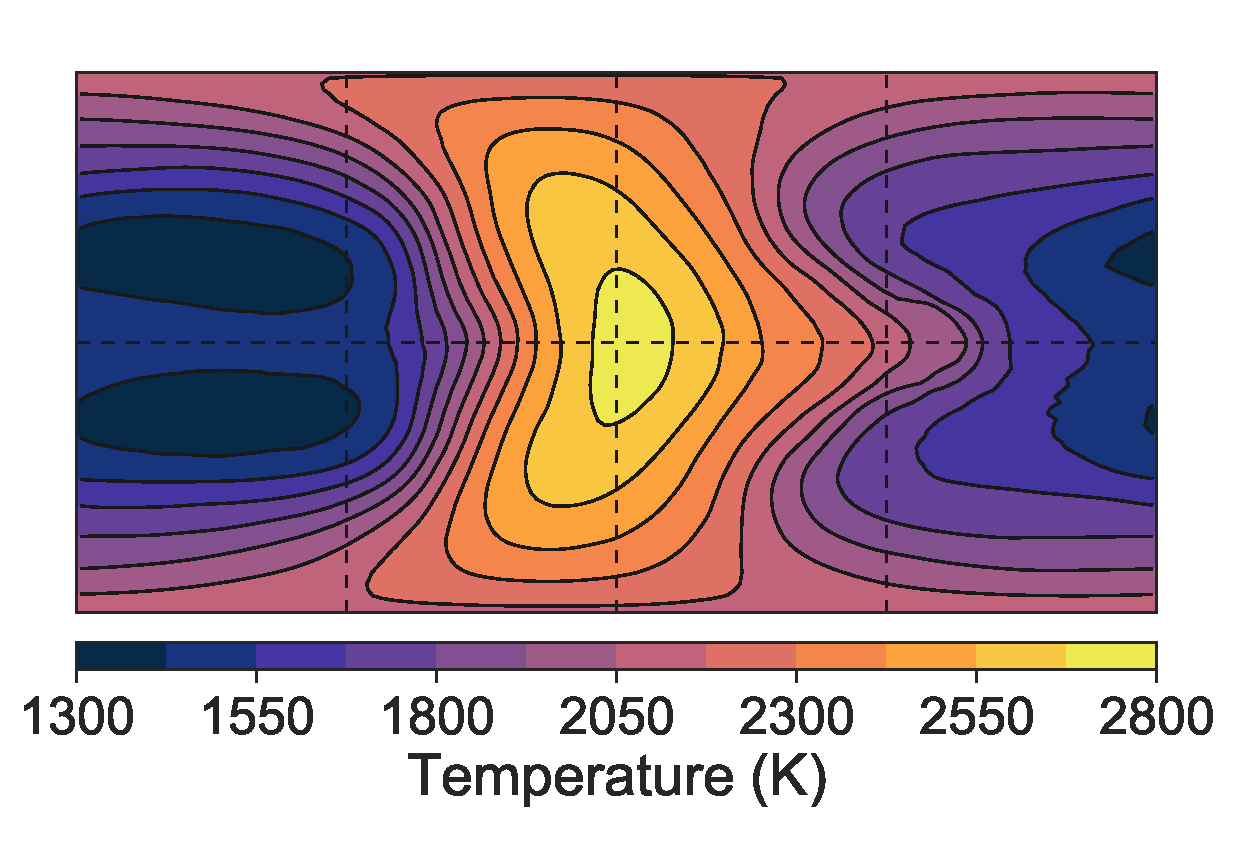
\includegraphics[width=\textwidth]{figures/linking-climate-55cnce/N2_brightT.eps}
    \caption{Test 2 brightness.}
    \label{fig:free-h-shear}
  \end{subfigure}
  \\
  \begin{subfigure}[t]{0.32\textwidth}
    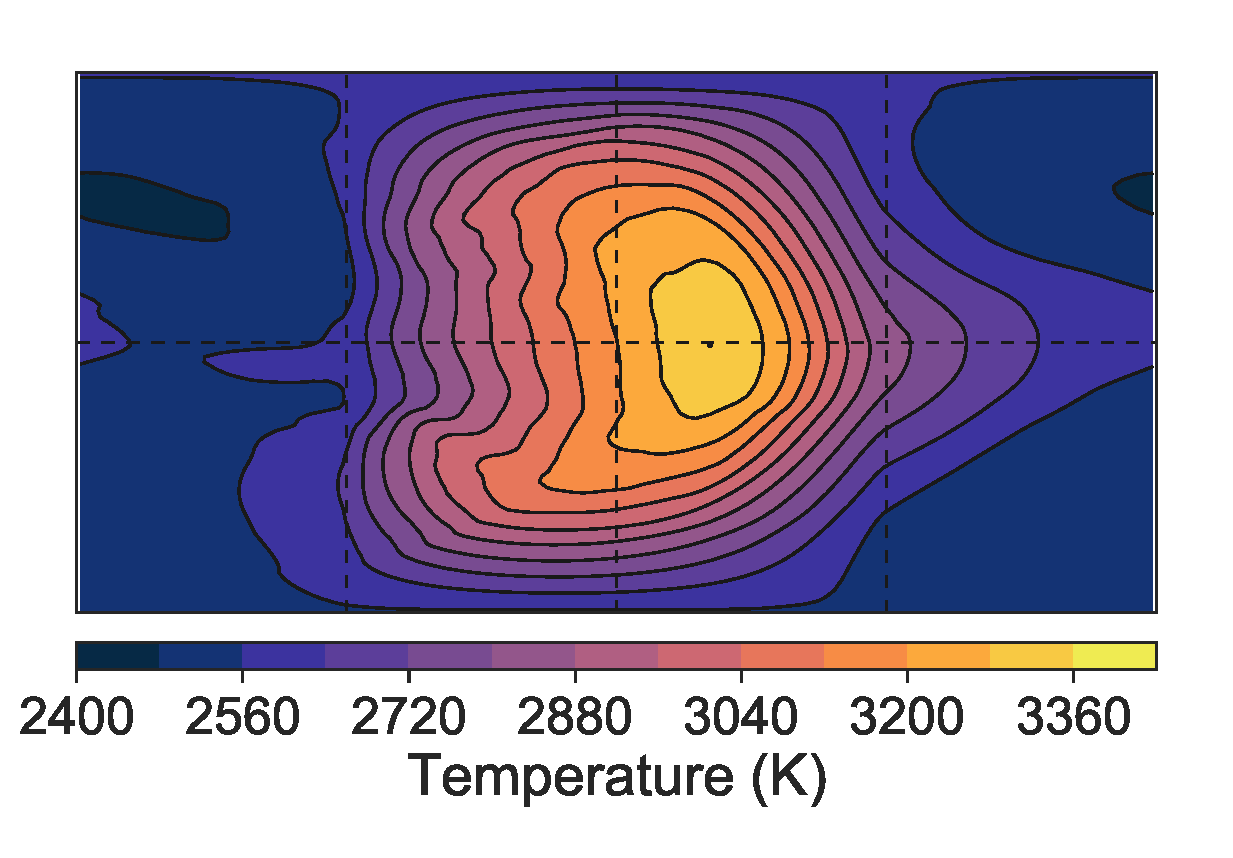
\includegraphics[width=\textwidth]{figures/linking-climate-55cnce/10sh_surfp.eps}
    \caption{Test 3 surface.}
    \label{fig:free-u-shear}
  \end{subfigure}
\enskip
  \begin{subfigure}[t]{0.32\textwidth}
    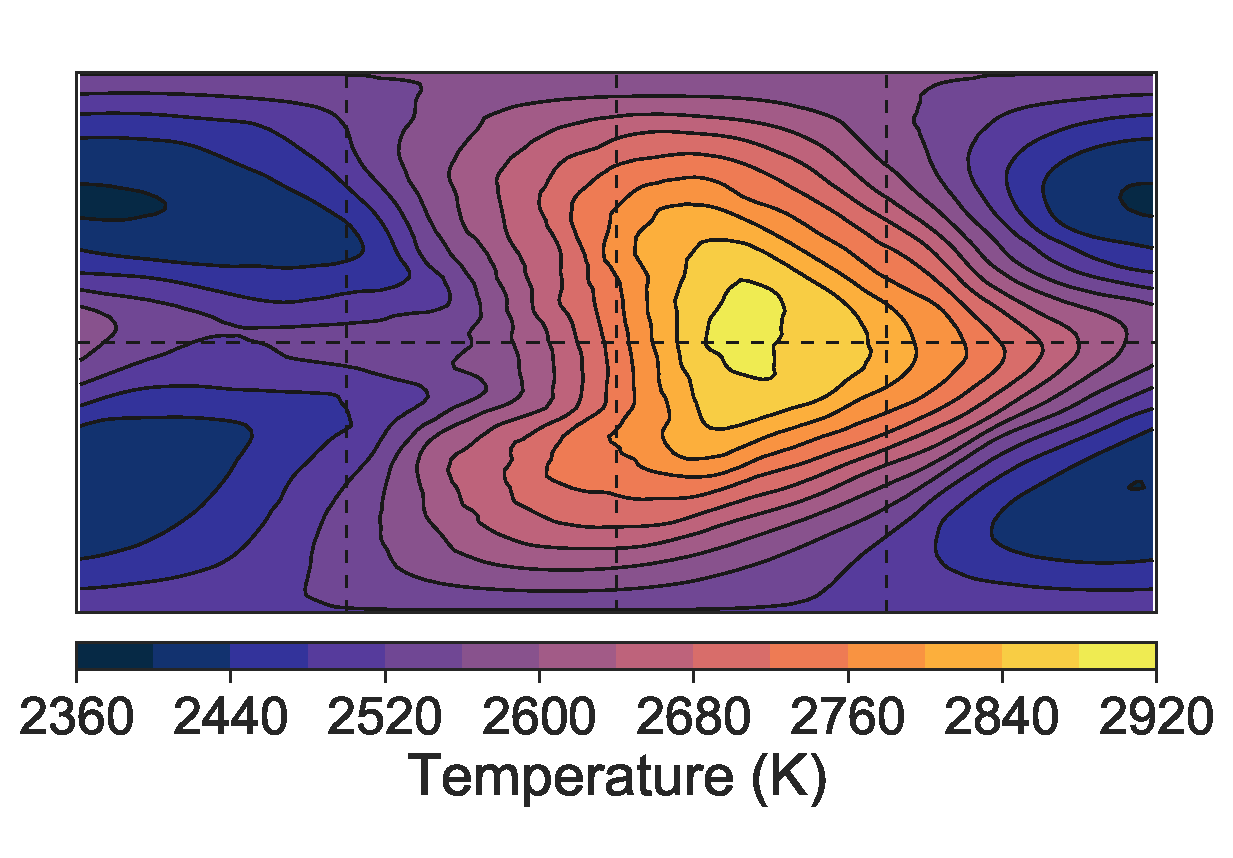
\includegraphics[width=\textwidth]{figures/linking-climate-55cnce/10sh_halfp.eps}
    \caption{Test 3 mid-atmosphere.}
    \label{fig:free-v-shear}
  \end{subfigure}
\enskip
  \begin{subfigure}[t]{0.32\textwidth}
    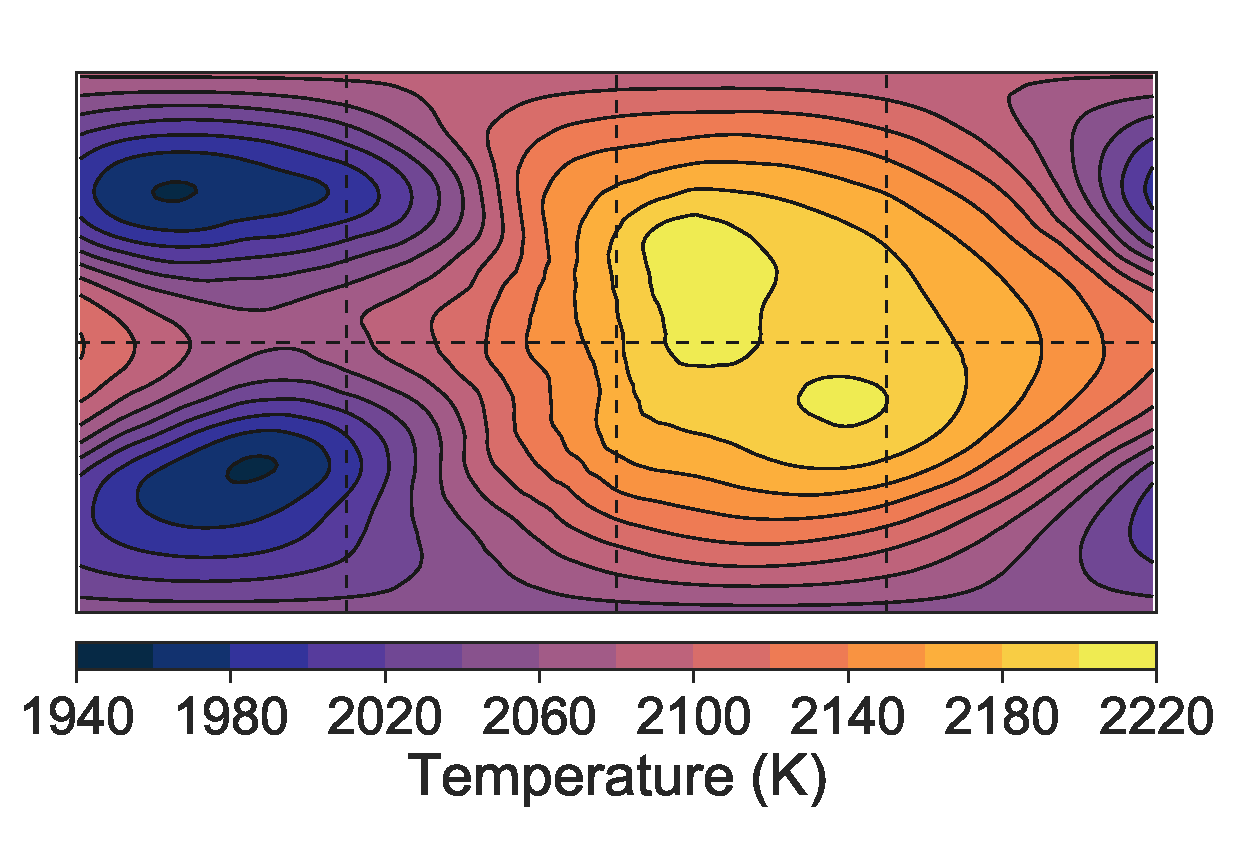
\includegraphics[width=\textwidth]{figures/linking-climate-55cnce/10sh_brightT.eps}
    \caption{Test 3 brightness.}
    \label{fig:free-h-shear}
  \end{subfigure}
  \caption{10-day time-averaged maps of different temperature fields for Tests 1, 2, and 3. Each row is a different test. The first column shows the surface air temperature, which has the strongest day-night contrast as it is closely coupled to the surface temperature and stellar forcing. The second column is the temperature at the half-surface-pressure level, which can support both a large hot-spot shift and day-night contrast. The third column is the brightness temperature calculated from the semi-grey radiative transfer scheme, which generally corresponds to a low atmospheric pressure, due to the high optical thickness.}
  \label{fig:Tlevels-maps}
\end{figure}




%SUBSECTION --
\subsection{Effect of Surface Pressure}\label{sec:ps_effect}

This section investigates the effect of the surface pressure on the global circulation. Section \ref{sec:scaling-relations} predicts that the surface pressure has a similar effect to the mean molecular weight, as they both modify the radiative timescale. At low surface pressures, the radiative timescale is short so there should be a large day-night contrast and small hot-spot shift, and vice versa. The surface pressure and the specific heat capacity have a similar effect, as they both affect the radiative timescale in the same way in Section \ref{sec:scaling-relations}.

Figure \ref{fig:H2N2_T_maps} shows the temperature at the half-surface-pressure level for these tests. The first row shows Tests 4, 5, and 6, with $\mu =$ \SI{4.6}{\gram\per\mole} and $p_{s} = 10$, $5$, and $3\ \mathrm{bar}$. As expected, the tests with higher $p_{s}$ have a larger hot-spot shift and smaller day-night contrast. The second row shows Tests 7, 8, and 9 with $\mu = $ \SI{15.0}{\gram\per\mole} and $p_{s} = 10$, $5$, and $3\ \mathrm{bar}$. Again, the tests with higher $p_{s}$ have a larger hot-spot shift and smaller day-night contrast. In comparison with the corresponding tests in the first row, all these tests have a larger day-night contrast and smaller hot-spot shift due to their higher mean molecular weight.

Test 3, with $\mu =$ \SI{4.6}{\gram\per\mole} and $p_{s} = 10\ \mathrm{bar}$, is consistent with the hot-spot shift and day-night contrast of the observed phase curve, but has a hotter night-side than the observations. Test 4 with $\mu =$ \SI{4.6}{\gram\per\mole} and $p_{s} = 5\ \mathrm{bar}$ is a better fit as it matches the day-side of the observations, and comes closer to matching the night-side. So, I will consider Test 4 with $p_{s} = 5\ \mathrm{bar}$ to be the ``best-fit'' test (although none of the simulations exactly matched the observations).

The simulations show that a low mean molecular weight of $\mu =$ \SI{2.0}{\gram\per\mole} or below cannot be consistent with the observations as the day-night contrast would be too small, as predicted by the scaling relations of \citet{zhang2017dynamics}. They also show that a high mean molecular weight of $\mu=$ \SI{28.0}{\gram\per\mole} or above does not fit the observations (in this range of surface pressures) as the hot-spot shift would be too small. Chapter \ref{ch:clouds-lava-planets} will investigate a larger range of pressures and consider the possibility of a higher mean molecular weight atmosphere. In the current chapter, the simulations suggest an atmosphere which is heavier than $\mu=$ \SI{2.0}{\gram\per\mole}, with a surface pressure in the range 1 to 10 bar. These conclusions are similar to other studies using different observations and models \citep{winn2011super, angelo201755cnce}.

The rest of this chapter discusses the effect of the longwave optical thickness and other bulk parameters on the circulation and vertical structure of the atmosphere. I will suggest that night-side cloud formation could be responsible for the low temperatures observed on the night-side, which would explain why the GCM simulations are consistently too hot on their night-sides.


\begin{figure}
  \begin{subfigure}[t]{0.33\textwidth}
    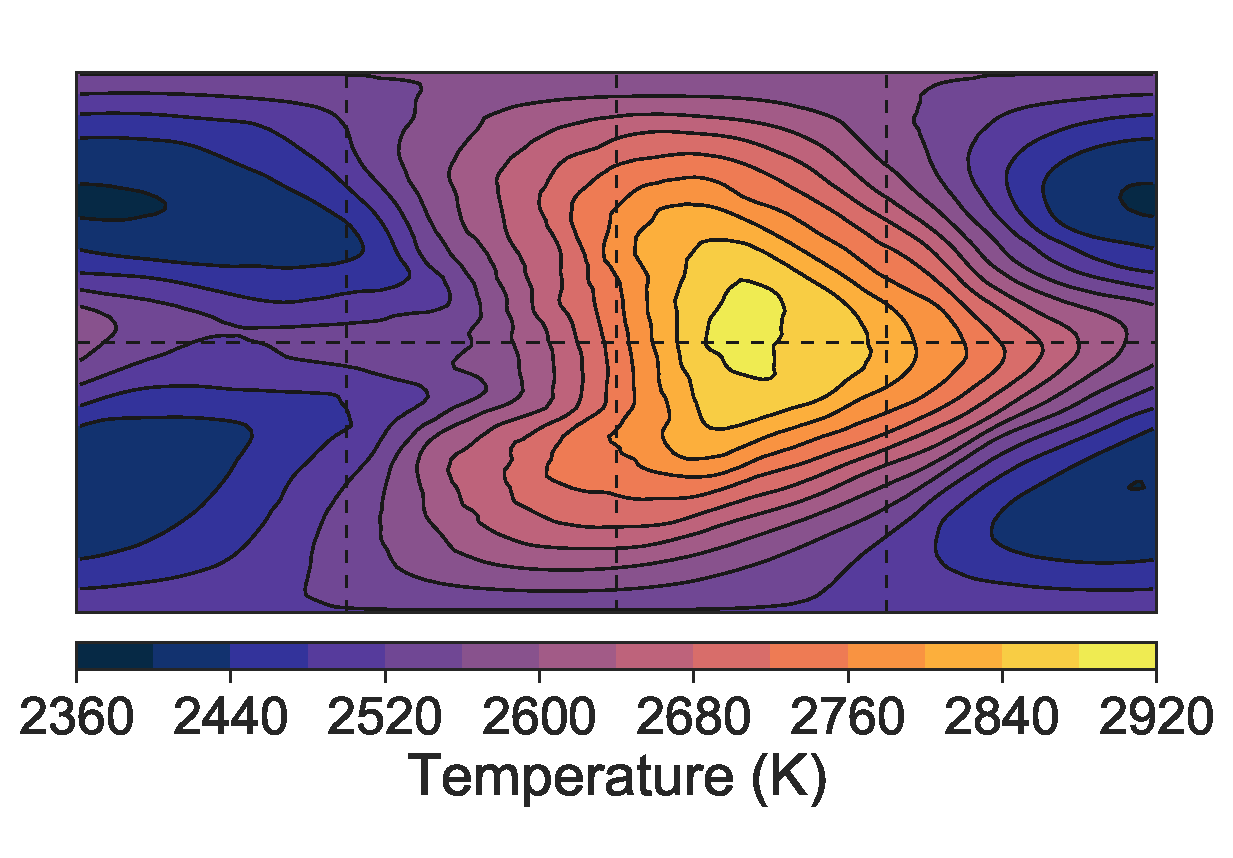
\includegraphics[width=\textwidth]{figures/linking-climate-55cnce/H2N2_10_halfp.eps}
    \caption{Test 3: \SI{4.6}{\gram\per\mole}, 10 bar}
    \label{fig:free-u-shear}
  \end{subfigure}
  %
  \begin{subfigure}[t]{0.33\textwidth}
    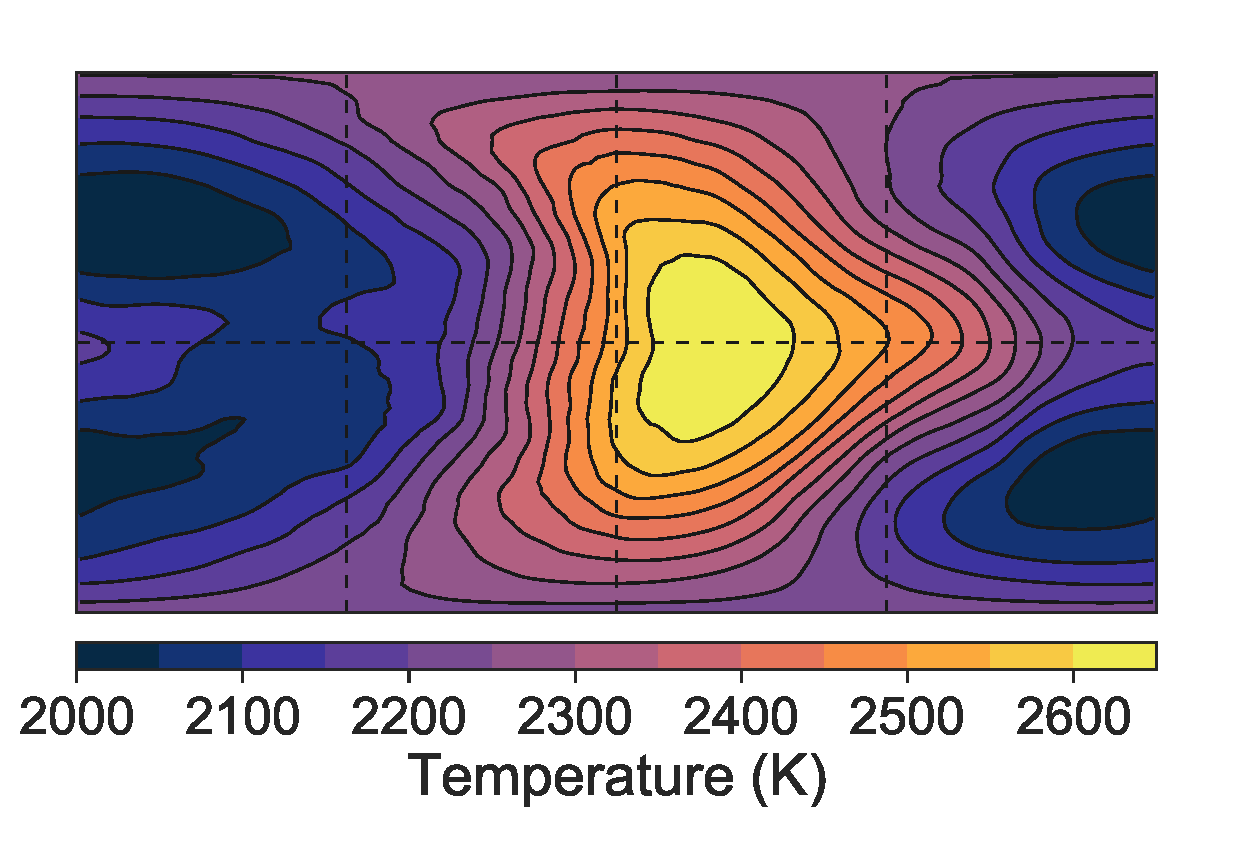
\includegraphics[width=\textwidth]{figures/linking-climate-55cnce/H2N2_5_halfp.eps}
    \caption{Test 4: \SI{4.6}{\gram\per\mole}, 5 bar}
    \label{fig:free-v-shear}
  \end{subfigure}
  %
  \begin{subfigure}[t]{0.33\textwidth}
    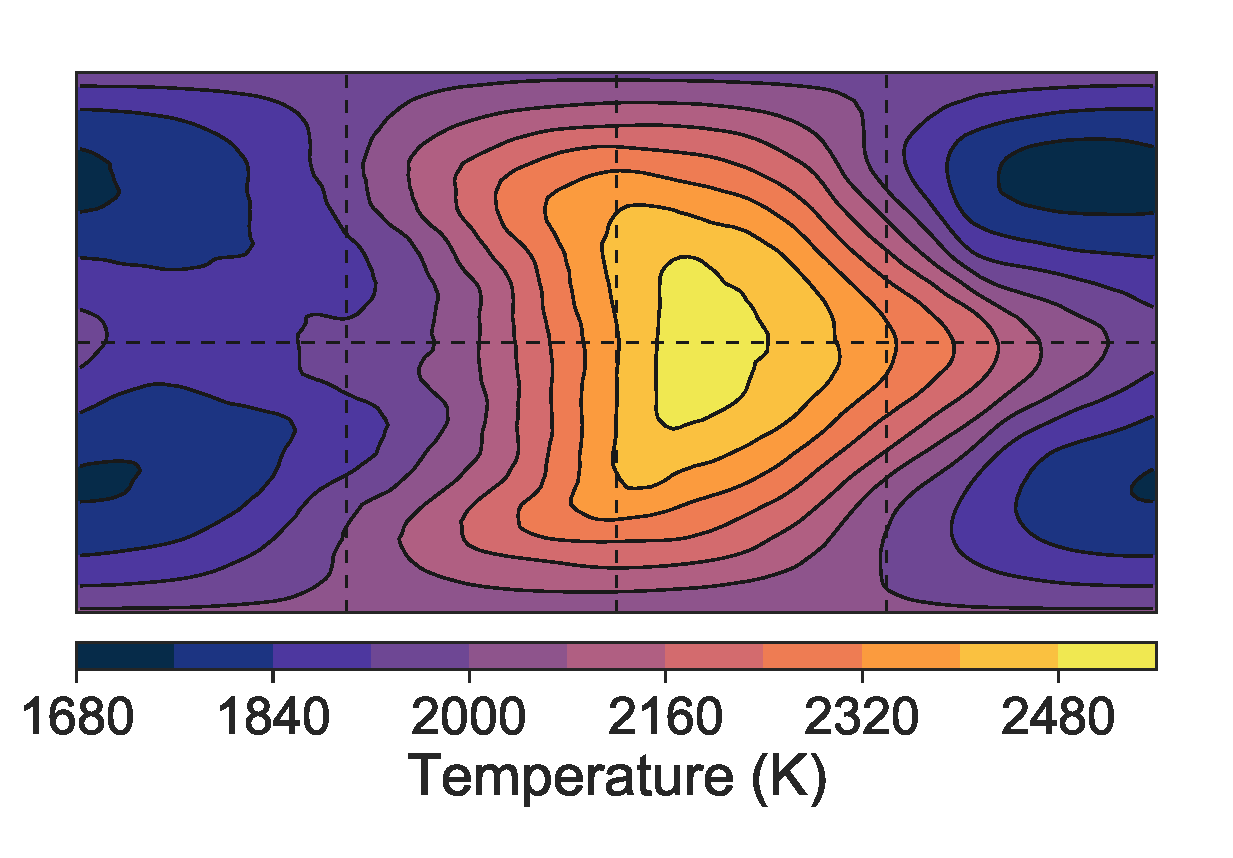
\includegraphics[width=\textwidth]{figures/linking-climate-55cnce/H2N2_3_halfp.eps}
    \caption{Test 5: \SI{4.6}{\gram\per\mole}, 3 bar}
    \label{fig:free-h-shear}
  \end{subfigure}
  \\
  \begin{subfigure}[t]{0.33\textwidth}
    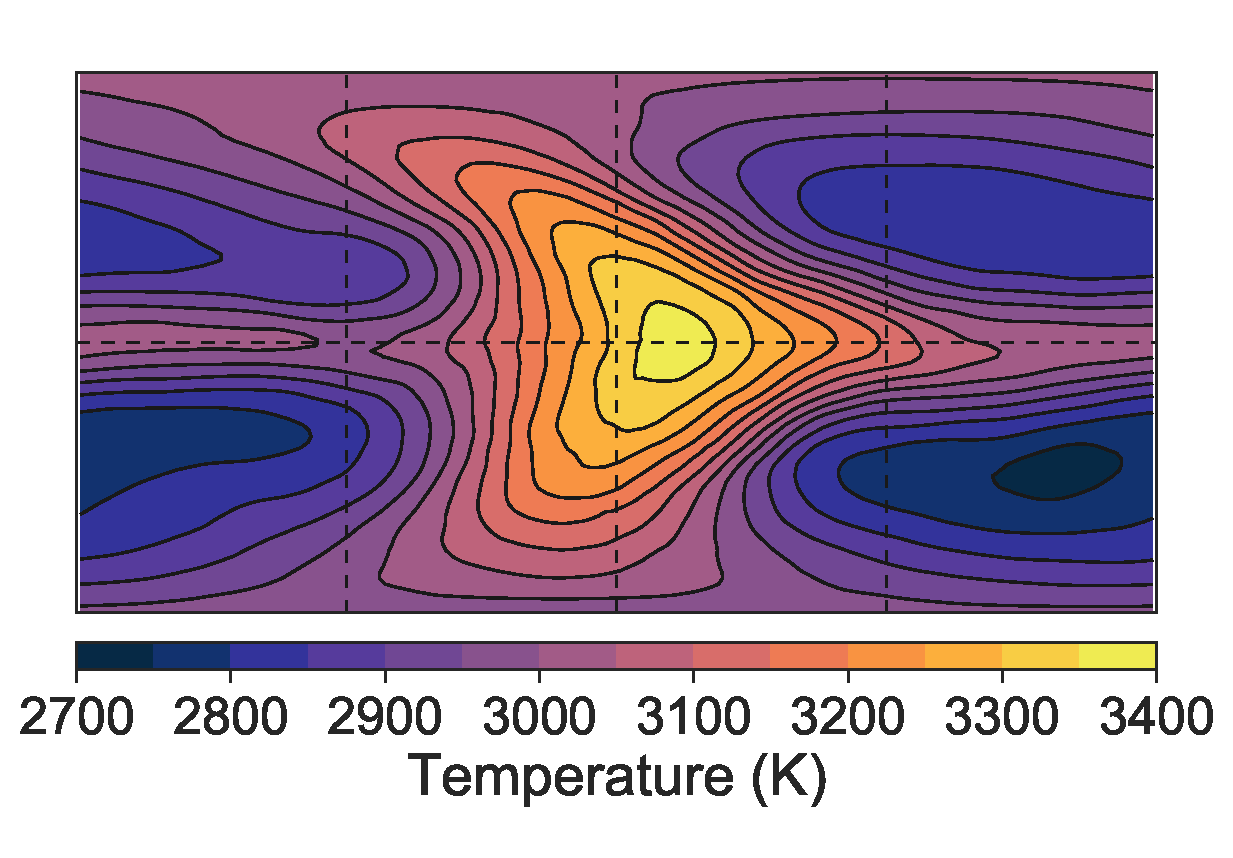
\includegraphics[width=\textwidth]{figures/linking-climate-55cnce/15GMOL_10_halfp.eps}
    \caption{Test 6: \SI{15.0}{\gram\per\mole}, 10 bar}
    \label{fig:free-u-shear}
  \end{subfigure}
  %
  \begin{subfigure}[t]{0.33\textwidth}
    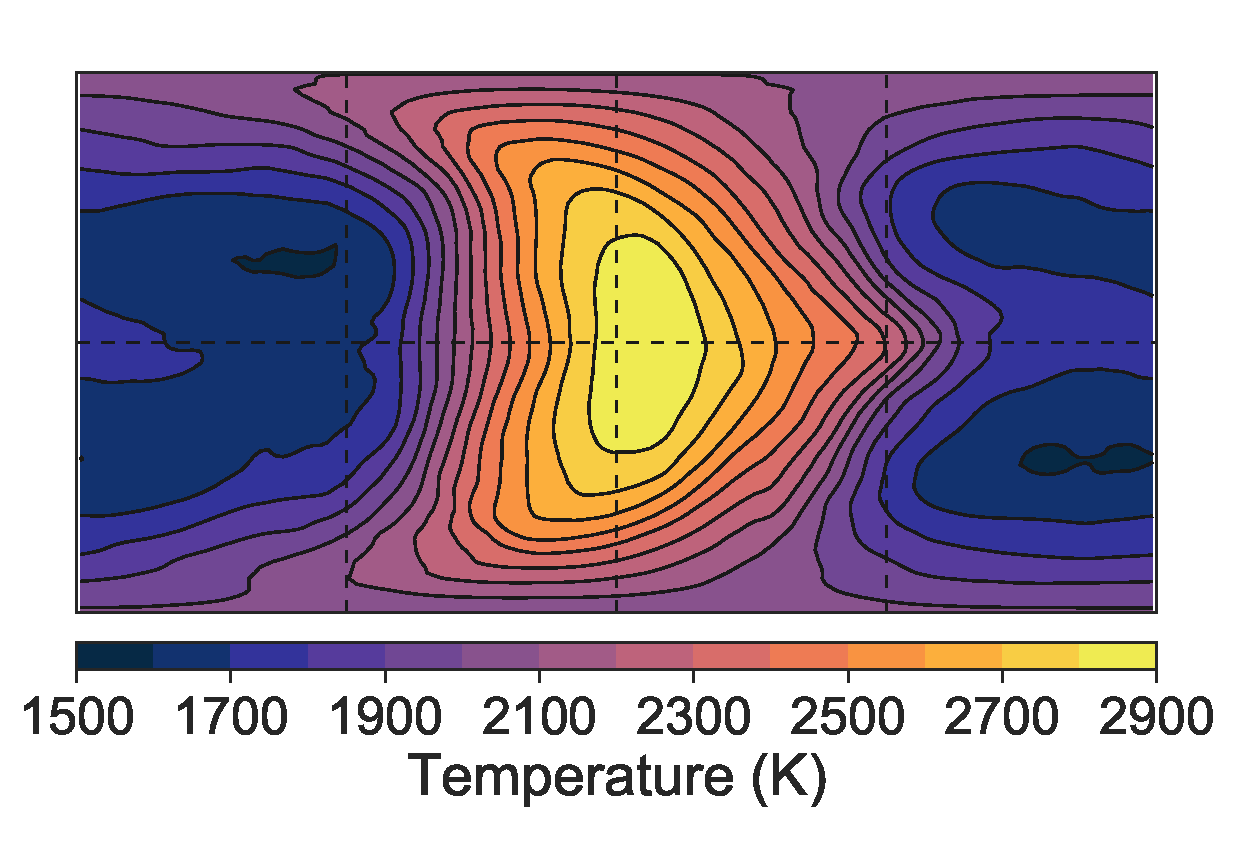
\includegraphics[width=\textwidth]{figures/linking-climate-55cnce/15GMOL_5_halfp.eps}
    \caption{Test 7: \SI{15.0}{\gram\per\mole}, 5 bar}
    \label{fig:free-v-shear}
  \end{subfigure}
  %
  \begin{subfigure}[t]{0.33\textwidth}
    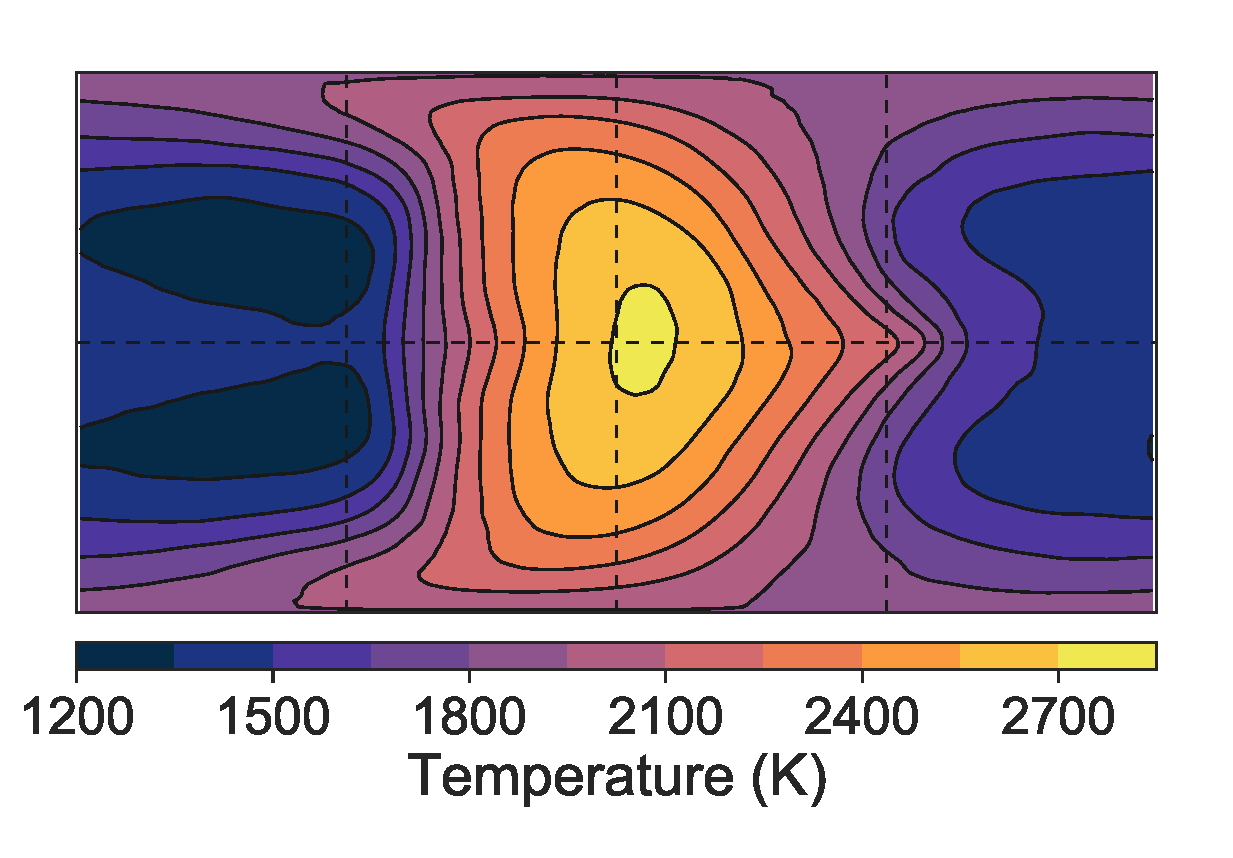
\includegraphics[width=\textwidth]{figures/linking-climate-55cnce/15GMOL_3_halfp.eps}
    \caption{Test 8: \SI{15.0}{\gram\per\mole}, 3 bar}
    \label{fig:free-h-shear}
  \end{subfigure}
  \caption{Temperatures at half-surface-pressure averaged over 10 days, for atmospheres with mean molecular weights of either $\mu =$ \SI{4.6}{\gram\per\mole} or \SI{15.0}{\gram\per\mole}, and surface pressures of 3, 5, or 10 bar.}
  \label{fig:H2N2_T_maps}
\end{figure}

%SUBSECTION --
\subsection{Effect of Optical Thickness}\label{sec:tauinf_effect}

This section will show that the main effect of changing the longwave optical thickness $\tau_{\infty}$ is to change the global mean temperature without strongly affecting the circulation and the shape of the phase curve. The high day-side brightness temperature observed by  \citet{demory201655cnce} requires significant greenhouse heating, which approximately constrains the longwave optical depth of the atmosphere.

Figure \ref{fig:vary_tau_maps} shows three atmospheres based on the ``best-fit'' Test 4. Tests 7, 8, and 9 have $p_{s} = 10\ \mathrm{bar}$ and $\mu =$ \SI{4.6}{\gram\per\mole}, with $\tau_{\infty} =$ 8.0, 4.0, and 2.0. Section \ref{sec:scaling-relations} predicts that $\tau_{\infty}$ will not have a large effect on the hot-spot shift and fractional day-night contrast, beyond scaling the global mean temperature. This is confirmed by Figure \ref{fig:vary_tau_maps}, where the temperature distributions have different magnitudes but similar patterns. The high day-side temperature of Test 11 matches the day-side temperature of the phase curve best, but its night-side temperature is much higher than the observations. The tests with lower optical thickness match the night-side observations better but the day-side observations worse. This is another example of the difficulty in fitting the observed phase curve, which appears to require a very specific atmospheric structure. These tests show that the longwave optical depth of the atmosphere must be in the range $\tau_{\infty} =$ 8.0 to 2.0, or the mean temperature of the atmosphere would be too high or too low. Figure \ref{fig:phasecurves_tauinf} will show later that varying $\tau_{\infty}$ just scales the magnitude of the thermal phase curves, with no significant differences in hot-spot shift or fractional day-night contrast.

\begin{figure}
  \begin{subfigure}[t]{0.32\textwidth}
    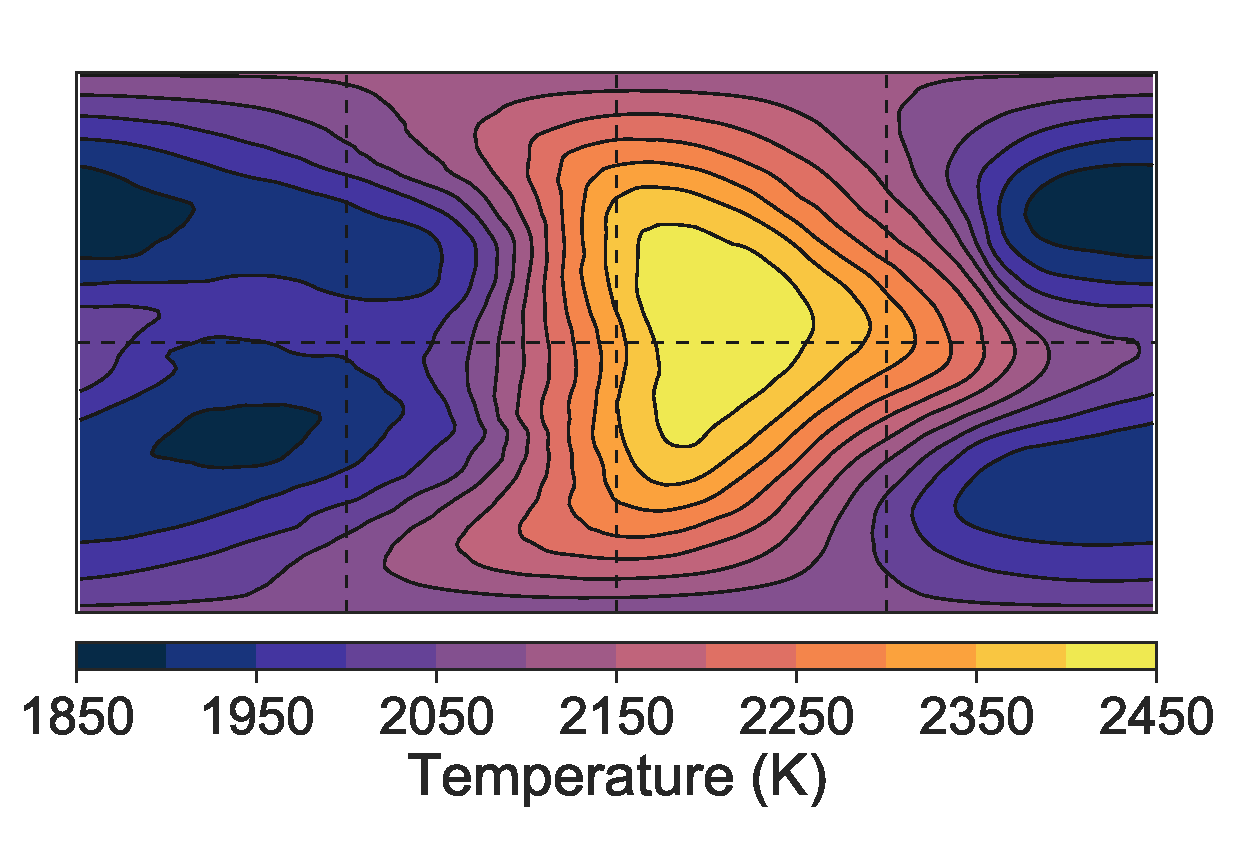
\includegraphics[width=\textwidth]{figures/linking-climate-55cnce/5sh_2_halfp.eps}
    \caption{Test 9, $\tau_{\infty} = 2.0$}
    \label{fig:free-u-shear}
  \end{subfigure}
\enskip
  \begin{subfigure}[t]{0.32\textwidth}
    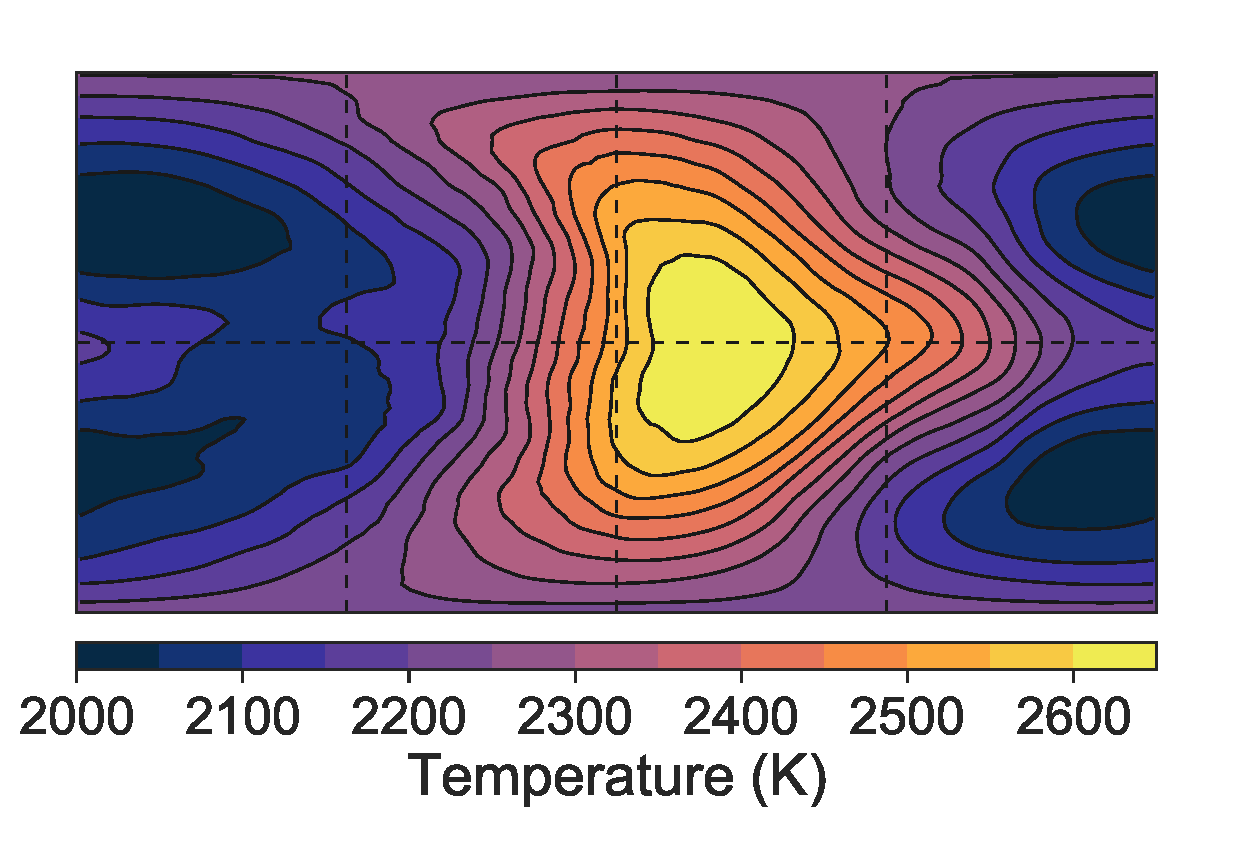
\includegraphics[width=\textwidth]{figures/linking-climate-55cnce/H2N2_5_halfp.eps}
    \caption{Test 10, $\tau_{\infty} = 4.0$.}
    \label{fig:free-v-shear}
  \end{subfigure}
\enskip
  \begin{subfigure}[t]{0.32\textwidth}
    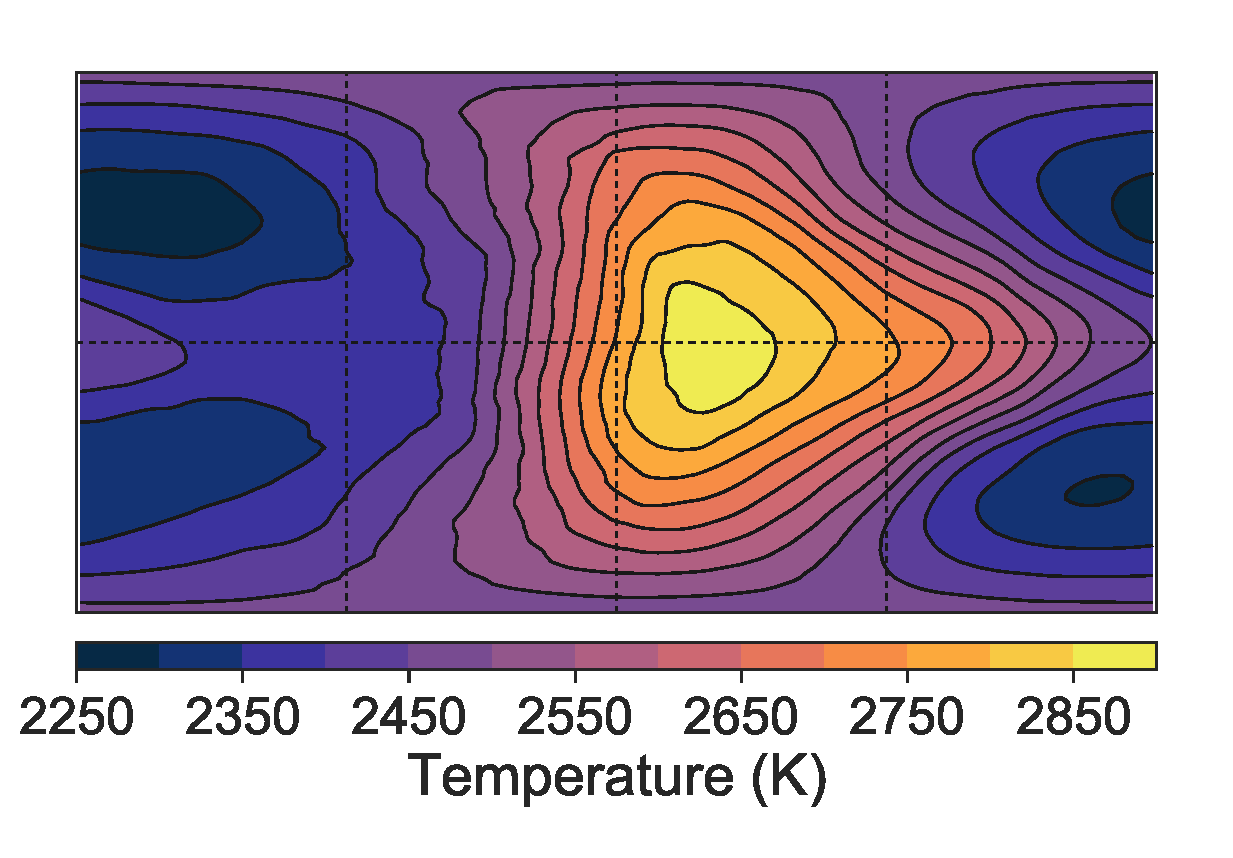
\includegraphics[width=\textwidth]{figures/linking-climate-55cnce/5sh_8_halfp.eps}
    \caption{Test 11, $\tau_{\infty} = 8.0$.}
    \label{fig:free-h-shear}
  \end{subfigure}
  \caption{The temperature at the half-surface-pressure level for Tests 10, 11, and 12, with $\mu=$ \SI{4.6}{\gram\per\mole}, surface pressure 5 bar and optical thicknesses of 2.0, 4.0, and 8.0. Increasing the optical thickness increases the global mean temperature but does not significantly affect the global circulation and temperature distribution.}
\label{fig:vary_tau_maps}
\end{figure}

%SUBSECTION --
\subsection{Vertical Temperature Structure}\label{sec:vertical_structure}

The thermal phase curve that would result from any of these simulations depends on the radiative properties of the atmosphere in the wavelength range of the observations. This chapter will assume that the outgoing radiation can be approximated as the emission from a single pressure level in the atmosphere -- see Chapter \ref{ch:clouds-lava-planets} for more detailed modelling of the outgoing thermal emission.

The phase curve of the emission from a radiating level near the surface will have almost no hot-spot shift and a large day-night contrast, as it is closely coupled to the surface temperature which is dominated by the incoming shortwave stellar radiation. If the radiating level is very high in the atmosphere, the phase curve could be almost flat due to efficient circulation as in Test 1, or it could still have a large day-night contrast as in Test 2. Generally, to fit the observed large day-night contrast and large hot-spot shift the radiating level must be somewhere between these two extremes. In this section, I will examine the vertical structure of the test atmospheres, and discuss how the observable quantities vary with pressure level.

Figure \ref{fig:tp-profiles} shows temperature-pressure profiles of several vertical columns spaced evenly around the equator of Test 4. The red line at the substellar point is convective at high pressures, driven by the stellar heating at the surface. The blue line at the east terminator has a temperature inversion above the lower atmosphere, caused by the hot-spot shift that is strongest at the level of the equatorial jet at approximately $0.5\ \mathrm{p_{s}}$. It might be possible to detect an inversion due to atmospheric dynamics on a tidally locked planet with a strong circulation with phase-resolved emission spectroscopy \citep{stevenson2014thermal}. The temperature profile at the antistellar point is almost isothermal, as it is heated high in the atmosphere by the global circulation, rather than at the surface. These profiles show that the observable day-night contrast depends on the radiating level and thermal structure, as at the surface the temperature profiles are well separated but at low pressure they are almost uniform.

Figure \ref{fig:dnc-pressure} plots the day-night contrast at each pressure level in the atmosphere for Tests 1, 2, and 4. This suggests that the large observed day-night contrast corresponds to a radiating level near the surface. However, the high longwave optical thickness in the GCM means that the outgoing radiation in the model comes from high in the atmosphere, as shown in Figure \ref{fig:Tlevels-maps}. I will show later that the phase curves calculated from the outgoing radiation in the semi-grey scheme always have a day-night temperature contrast that is smaller than the observations. This suggests that in reality the atmospheric longwave thickness is high to explain the observed day-side temperature, but that the \SI{4.5}{\micro\metre} band corresponds to a region of lower absorption with a radiating level low in the atmosphere to explain the large day-night contrast.

Figure \ref{fig:hss-pressure} shows how the hot-spot shift varies with atmospheric pressure. It is always small close to the surface, where the temperature is closely coupled to the incoming stellar radiation due to the lack of shortwave absorption in these simulations. The hot-spot shift generally increases with height, as the zonal flow increases further from the surface up to a maximum at the centre of the jet. The heat redistribution can be so effective high in the atmosphere that it becomes almost isothermal, as shown by the brightness temperature of Test 1 in Figure \ref{fig:Tlevels-maps}.

The next section will investigate the same effects of atmospheric parameters on the global circulation by simulating the phase curves of each test. These will show the same trends as this section, and confirm the predictions of the scaling relations of \citet{zhang2017dynamics}.

\begin{figure}
  \begin{subfigure}[t]{0.32\textwidth}
    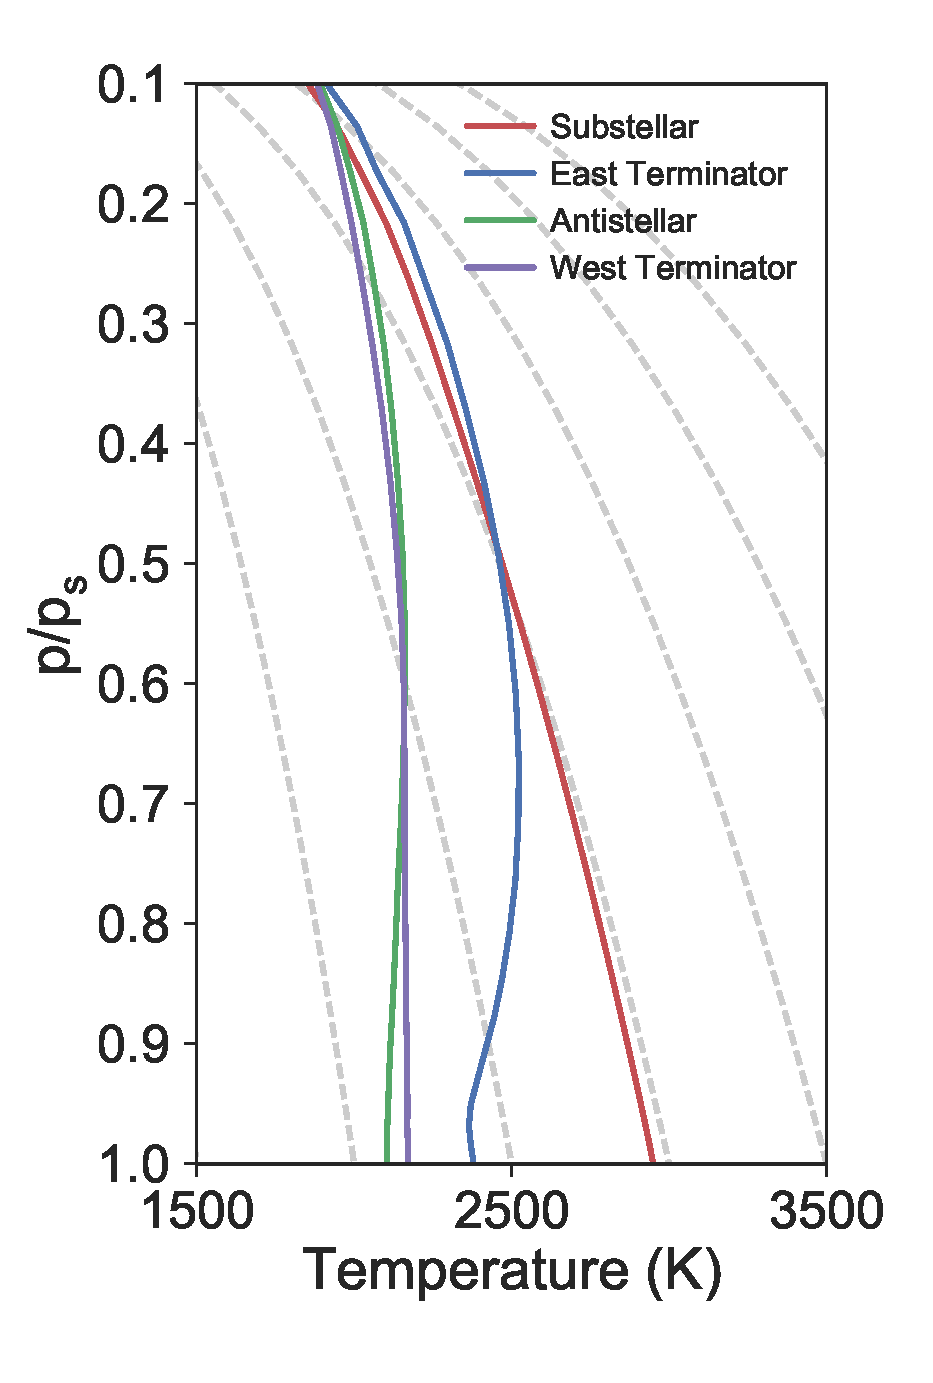
\includegraphics[width=\textwidth]{figures/linking-climate-55cnce/Tprofiles.eps}
    \caption{T(p) profiles for columns on the equator of Test 4. Dry adiabats are plotted in grey.}
    \label{fig:tp-profiles}
  \end{subfigure}
\enskip
  \begin{subfigure}[t]{0.32\textwidth}
    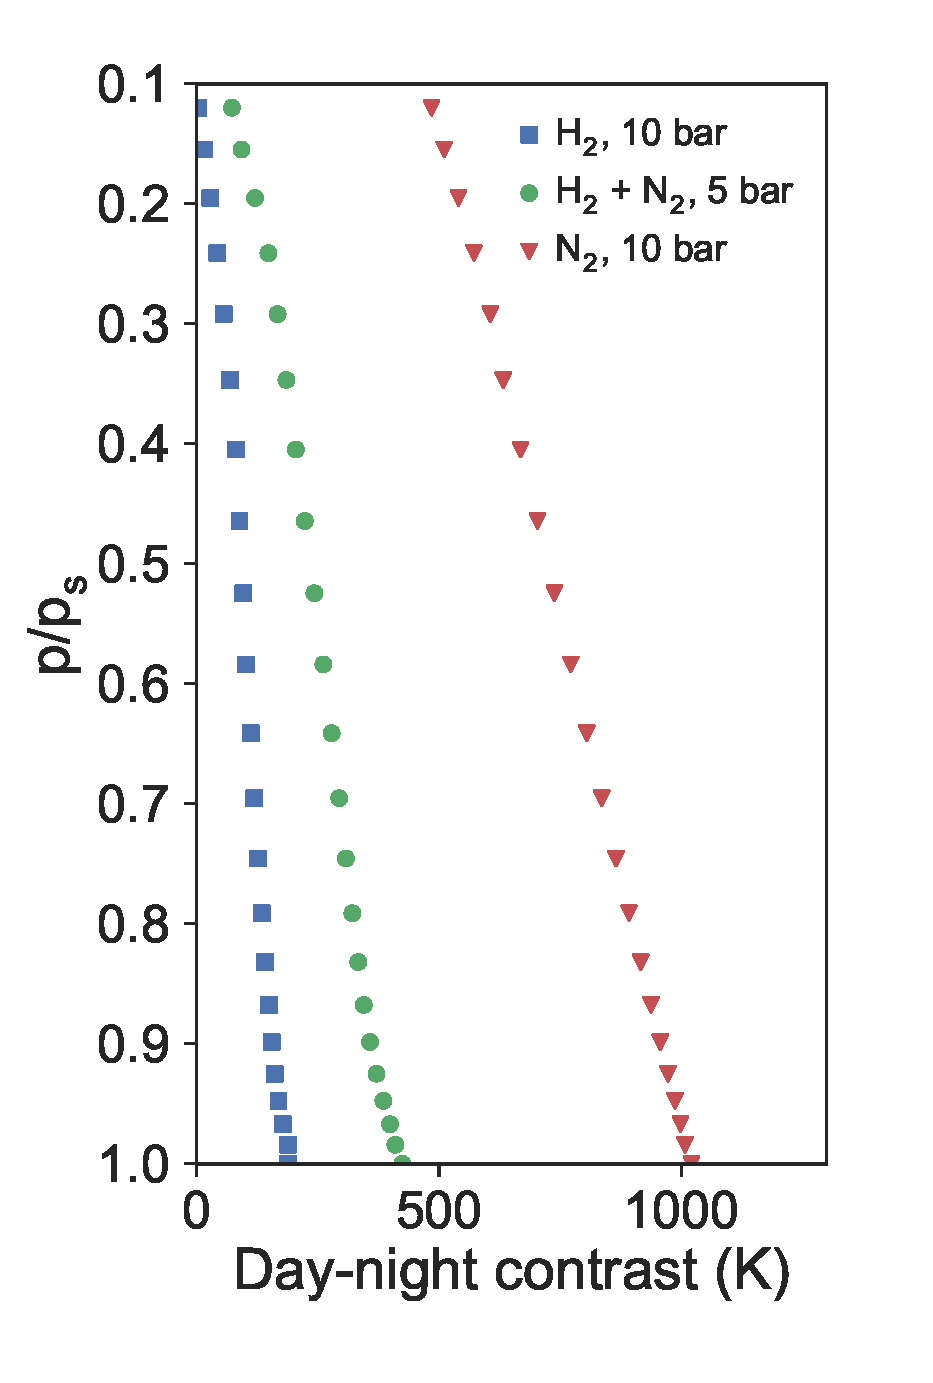
\includegraphics[width=\textwidth]{figures/linking-climate-55cnce/dncontrast.eps}
    \caption{Day-night contrast at each pressure level, showing how it is larger at higher pressures..}
    \label{fig:dnc-pressure}
  \end{subfigure}
\enskip
  \begin{subfigure}[t]{0.32\textwidth}
    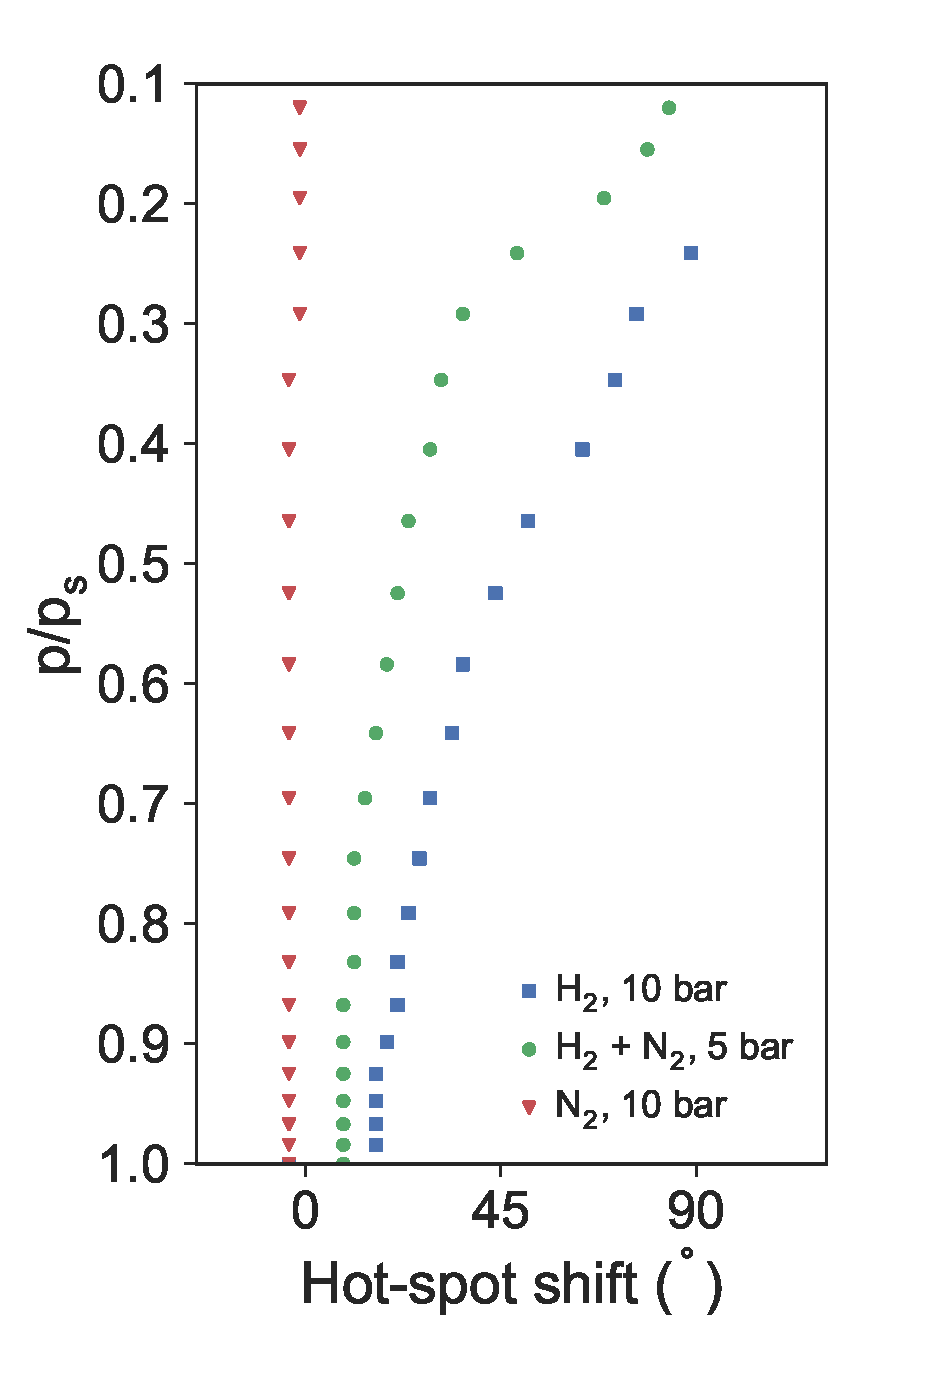
\includegraphics[width=\textwidth]{figures/linking-climate-55cnce/hotspotlocation.eps}
    \caption{Hot-spot shift at each pressure level, showing how it increases with height.}
    \label{fig:hss-pressure}
  \end{subfigure}
  \caption{The vertical structure of Test 4, and the hot-spot shift and day-night contrast of Tests 1, 2, and 4. The temperature profiles tend to follow the dry adiabat at high pressures on the day-side, but can become isothermal or inverted on the night-side. The lower atmospheres have a larger day-night contrast, and the upper atmospheres have a larger hot-spot shift. This suggests that the observed phase curve corresponds to emission from an intermediate pressure level.}
\label{fig:pressure_variation}
\end{figure}



%% UP TO HERE

%SECTION CONCLUSIONS



%%%%%%%%%%%%%%%%%%%%%%%%%%%%%%%%%%%%
%SECTION 5 -- OBSERVATIONS
\section{Simulated Observations}\label{sec:simulated-obs}

This section will discuss phase curves calculated from the GCM simulations shown previously. The \SI{4.5}{\micro\metre} phase curves were calculated using either the outgoing longwave radiation from the grey-gas model, or for a specific radiating level using the temperature of that level. This flux was integrated over the hemisphere centred on each grid cell around the equator, to produce the phase curve \citep{cowan2008inverting}:

\begin{equation}
  I_{p}(\xi) = \frac{\int_{-\pi/2}^{\pi/2} \int_{-\xi-\pi/2}^{-\xi+\pi/2}I_{4.5}^{\uparrow}|_{p=0}\cos(\lambda+\xi)\cos^{2}(\theta)d \lambda d \theta}{\int_{-\pi/2}^{\pi/2} \int_{-\xi-\pi/2}^{-\xi+\pi/2}\cos(\lambda+\xi)\cos^{2}(\theta)d \lambda d \theta}
\end{equation}

where the phase angle is $\xi$, the outgoing \SI{4.5}{\micro\metre} flux is $I_{4.5}^{\uparrow}|_{p=0}$, longitude is $\lambda$, and latitude is $\theta$. The phase curves are plotted as a ratio of planetary flux $F_{p}$ to stellar flux $F_{\circledast}$:

\begin{equation}
  \frac{F_{p}}{F_{\circledast}} = \frac{I_{p}}{I_{\circledast}}\Big( \frac{r_{p}}{r_{\circledast}} \Big) ^{2}
\end{equation}

where the ratio of planetary radius to stellar radius is $\frac{r_{p}}{r_{*}} = 0.0187$ and the stellar emission is determined by its effective temperature of \SI{5196}{\kelvin} \citep{von201155}.

\subsection{Effect of Radiating Level}

Section \ref{sec:vertical_structure} showed how the hot-spot shift and day-night contrast vary with pressure level due to changes in stellar forcing, radiative timescale, and jet speed. Figure \ref{fig:phasecurves} shows phase curves calculated from the emission at \SI{4.5}{\micro\metre} of different radiating levels in Test 4, which show the same trends in hot-spot shift and day-night contrast as the analysis in Section \ref{sec:vertical_structure}.

% The figure shows this instead of the OLR from the model, as in reality the atmosphere will not be grey, and the \SI{4.5}{\micro\metre} radiation could correspond to any level.



%Both the wave-based mechanism of Chapter \ref{ch:wave-mean-flow} and the advection-based mechanism of \citet{zhang2017dynamics} explain this trend as due to the decreasing temperature and increasing radiative timescale at lower pressures.

The phase curve from a pressure level close to the surface has a large amplitude and small phase shift as explained previously. High in the atmosphere, the phase curve has a smaller amplitude and large phase shift. I will show later in Figure \ref{fig:phasecurves_flux} that the mean molecular weight and radiating level are somewhat degenerate in their effects on the phase curve, as they both affect the radiative timescale which then changes the day-night contrast and hot-spot shift in the same way. Figures \ref{fig:phasecurves} and \ref{fig:phasecurves_flux} show phase curves varying from a case with low amplitude and large phase shift, to a case with high amplitude and low phase shift.

% both show phase curves varying from a large amplitude, low phase shift curve to one with low amplitude and large phase shift. In the simple picture of \citet{zhang2017dynamics}, these have the same effect on the circulation as they affect the radiative timescale in the same way. This degeneracy is not too great a problem in this chapter, as the observed phase curve is so extreme that both the radiating level and mean molecular weight must be tightly constrained to come close to matching it.

Observations at multiple wavelengths corresponding to multiple radiating levels could break this degeneracy. As discussed earlier, it is possible to explain the high observed brightness temperature and large hot-spot shift if the atmospheric opacity in the \SI{4.5}{\micro\metre} \textit{Spitzer} bandpass is lower than average in the longwave region -- i.e., it is observed in a window. A broadband thermal phase curve would constrain the overall brightness temperature, and could be compared with the \SI{4.5}{\micro\metre} observations to test the prediction that they correspond to a window in the atmospheric opacity. Chapter \ref{ch:clouds-lava-planets} discusses these possibilities in more detail.

\begin{figure}
  \centering
    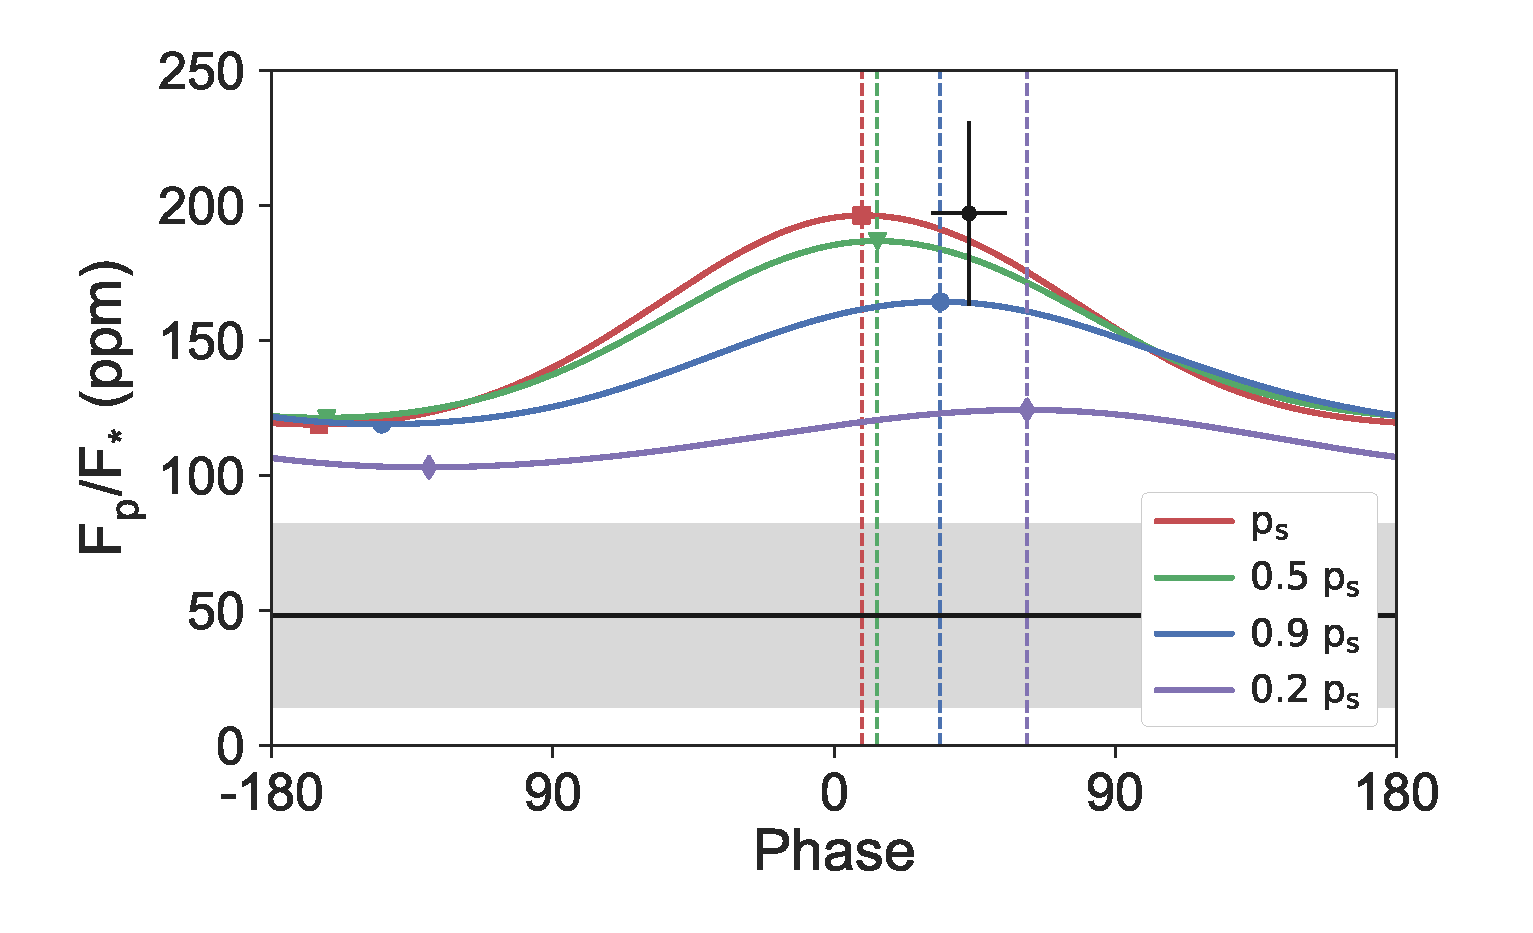
\includegraphics[width=0.75\textwidth]{figures/linking-climate-55cnce/phasecurves_p_level.eps}
    \caption{Thermal phase curves calculated at different radiating levels in Test 4. Moving the radiating level to lower pressures has a similar effect to decreasing the mean molecular weight, as shown in Figures \ref{fig:phasecurves_flux} and \ref{fig:phasecurves_temp}. The black point shows the maximum (day-side) observed flux, and the black line shows the minimum (night-side) observed flux.}
   \label{fig:phasecurves}
\end{figure}

\subsection{Effect of Atmospheric Properties}

Figure \ref{fig:phasecurves_flux} shows the phase curves of the simulated atmospheres with different values of mean molecular weight, calculated using the outgoing longwave radiation from each test. The black points show the maximum and minimum of the observed phase curve. The tests with very high or low molecular weight do not fit the observations well, as discussed previously. The phase curve of Test 1 (pure H\textsubscript{2}) has a large phase shift, but a very small amplitude due to its efficient heat transport from day-side to night-side. This can be explained using the wave-based theory in Chapter \ref{ch:wave-mean-flow}, as the low molecular weight would give a long radiative damping timescale, reducing the strength of the day-night wave-1 response, and producing a more zonally uniform temperature field like the solution in Figure \ref{fig:spherical-low-damp}.

The phase curve of Test 2 fits the day-night contrast but not the hot-spot shift, owing to its high radiative damping rate. The phase curve of Test 4 fits the observations better (as did its temperature distribution in Section \ref{sec:ps_effect}) -- it has a large amplitude and offset, although neither is quite as large as those in the observations. The relatively low amplitude of all the tests in Figure \ref{fig:phasecurves_flux} is due to the use of the model OLR in the phase curve. As discussed above, it may be that the observations at \SI{4.5}{\micro\metre} correspond to an atmospheric window, so actually reflect the temperature of a lower level in the atmosphere which would give a phase curve with a larger amplitude.



\begin{figure}
  \centering
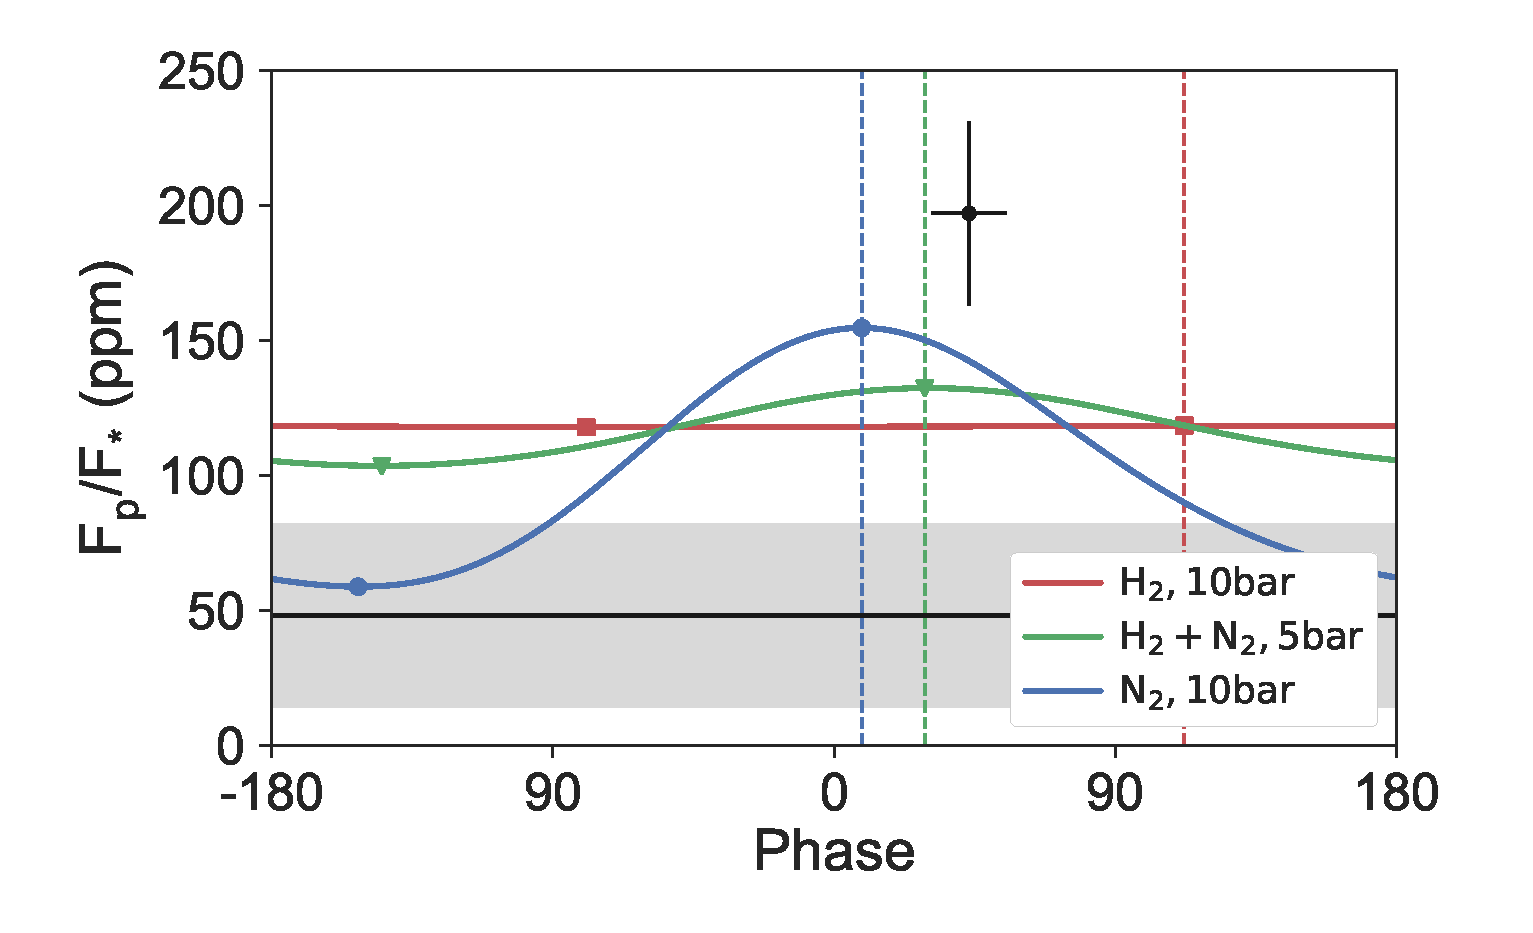
\includegraphics[width=0.75\textwidth]{figures/linking-climate-55cnce/phasecurves_flux.eps}
\caption{Simulated \SI{4.5}{\micro\metre} phase curves calculated from the grey-gas OLR of Tests 1, 2, and 4. The red curve is the Test 1, the 10 bar H\textsubscript{2} atmosphere, which has such efficient heat transport that it has a large peak offset and very small amplitude. The blue curve is Test 2, the 10 bar N\textsubscript{2} atmosphere, with very weak heat transport so a large amplitude and peak offset. The green curve is Test 4, the 5 bar H\textsubscript{2}+N\textsubscript{2} atmosphere, with a significant offset and amplitude. The offset and amplitude are not as large as the \citet{demory201655cnce} measurements, shown by the black point and line (with their errors shown by the bars and the shaded area).\label{fig:phasecurves_flux}}
\end{figure}

\begin{figure}
  \centering
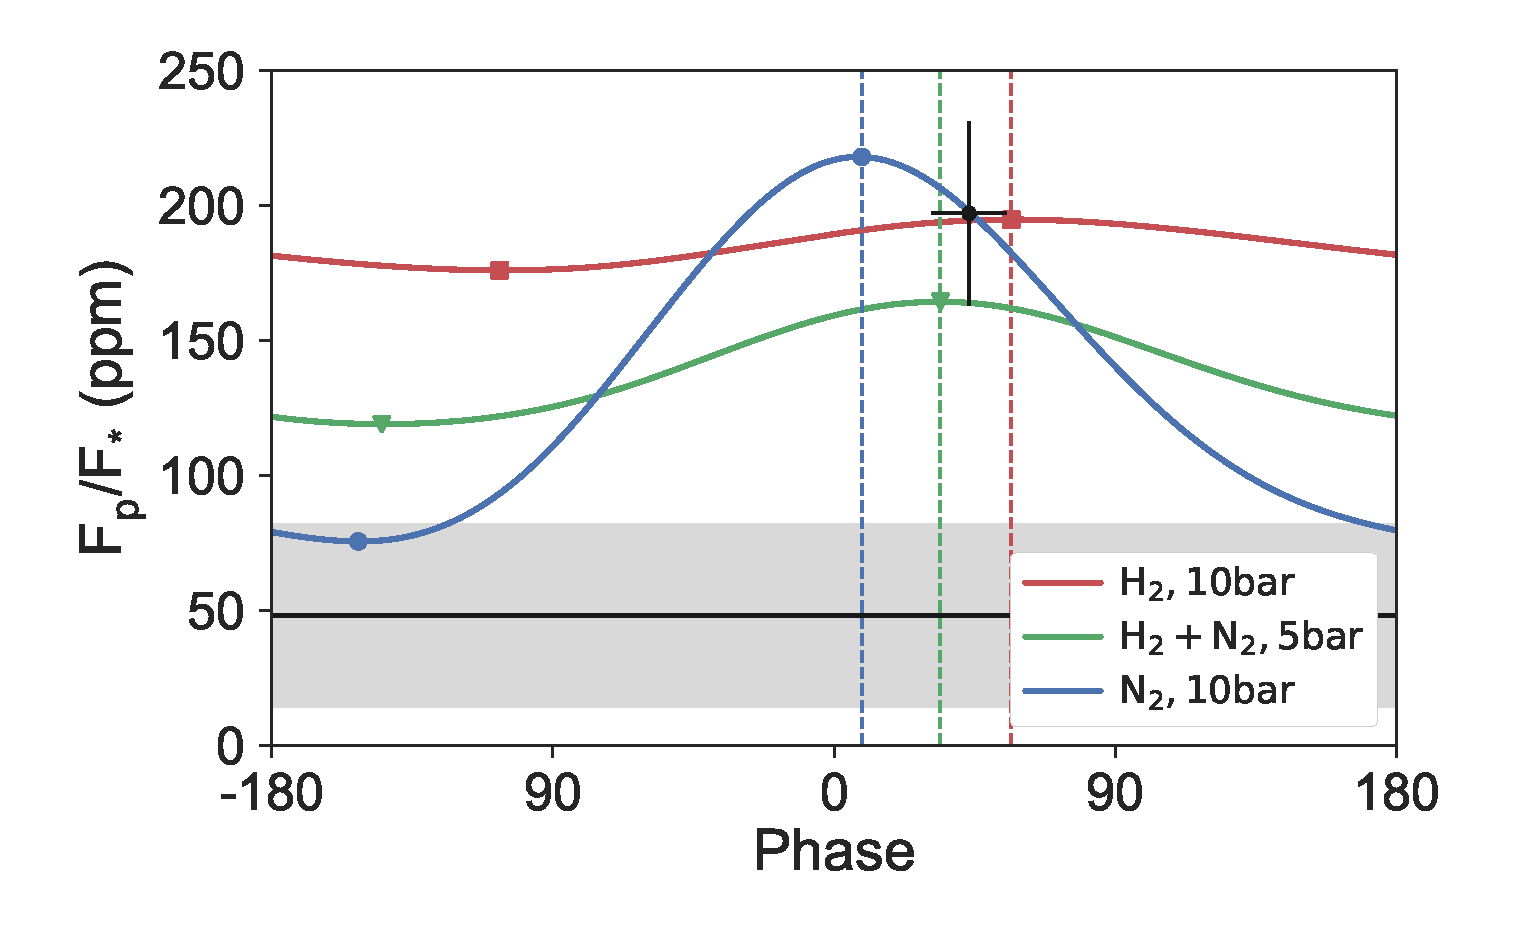
\includegraphics[width=0.75\textwidth]{figures/linking-climate-55cnce/phasecurves_temp.eps}
\caption{Simulated phase curves for the emission from a radiating level at half-surface-pressure for Tests 1, 2, and 4. The amplitude and offset are larger than the phase curves calculated from the OLR in Figure \ref{fig:phasecurves_flux}. The offset and amplitude are not as large as the \citet{demory201655cnce} measurements, but Figure \ref{fig:phasecurves_clouds} shows that the H\textsubscript{2}+N\textsubscript{2} atmosphere (green curve) could match the observations given night-side cloud formation as discussed in Section \ref{sec:condensables}.\label{fig:phasecurves_temp}}
\end{figure}

To test this idea, Figure \ref{fig:phasecurves_temp} shows the phase curves corresponding to the brightness temperature of a radiating level at half-surface-pressure for the same tests. Test 4 fits the observations better in this figure than in Figure \ref{fig:phasecurves_flux} where the model OLR was used. In this case, it has  a larger amplitude and a large phase shift due to the lower radiating level. The night-side flux is still higher than the observations as in most of the tests -- later, I will discuss the possibility of night-side cloud formation producing a difference between the model and the observations.

%
\begin{figure}
\centering
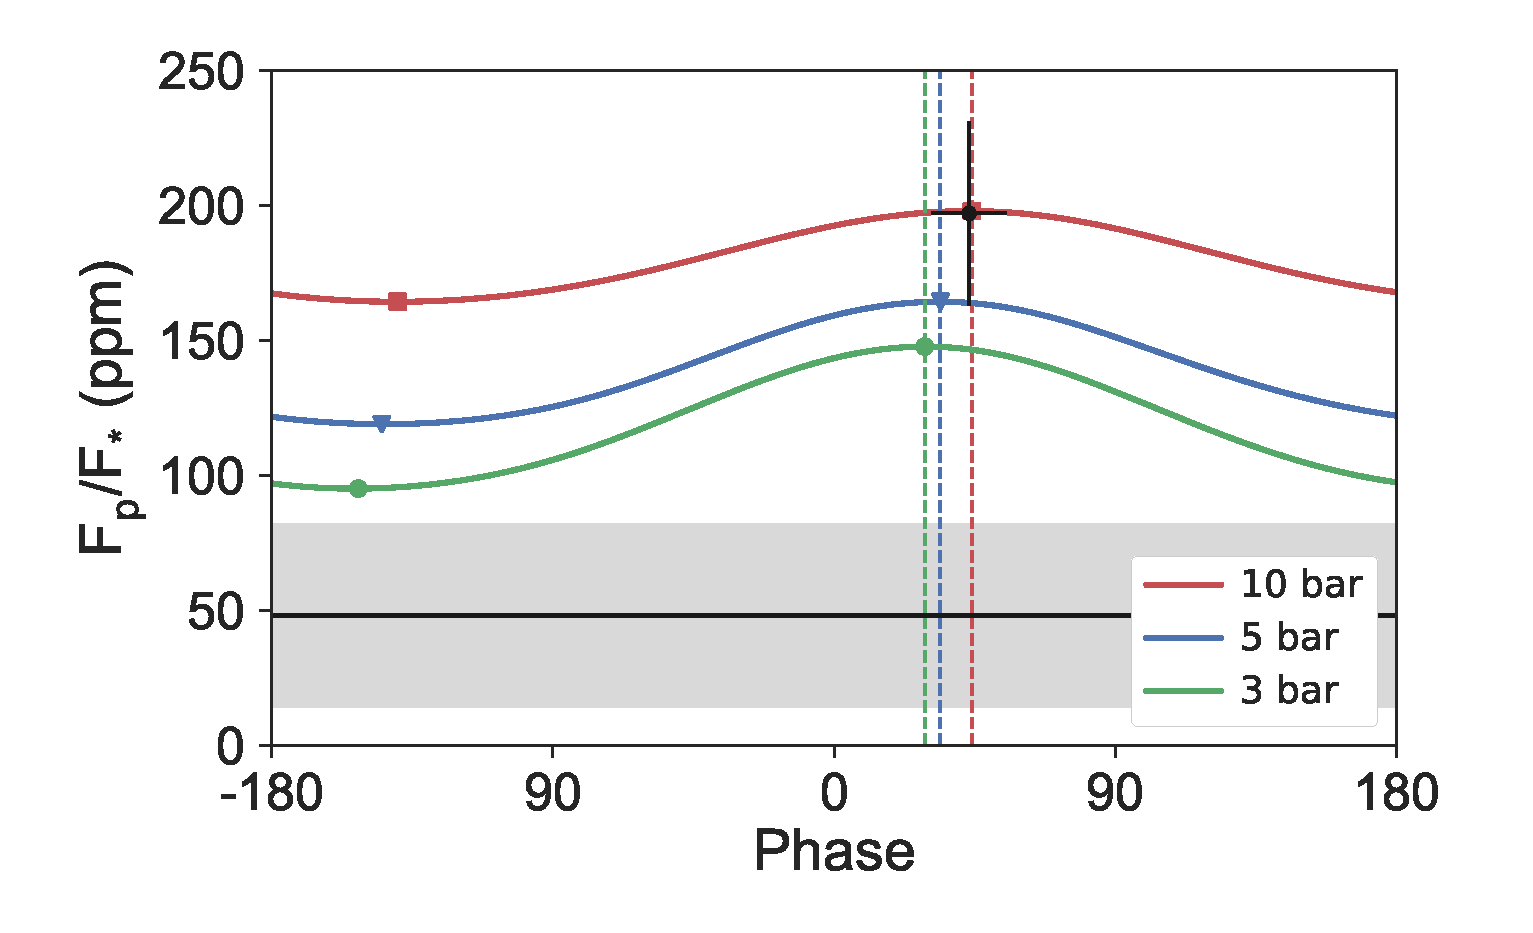
\includegraphics[width=0.75\textwidth]{figures/linking-climate-55cnce/phasecurves_vary_p.eps}
\caption{Phase curves calculated from the emission of the half-surface-pressure level of the \SI{4.6}{\gram\per\mole} H\textsubscript{2} + N\textsubscript{2} atmospheres (Tests 3, 4, and 5) with surface pressures of 3, 5, and 10 bar, corresponding to the temperature maps in Figure \ref{fig:H2N2_T_maps}.\label{fig:phasecurves_H2N2}}
\end{figure}


Figure \ref{fig:phasecurves_H2N2} shows the phase curves of the tests of different surface pressures in Section \ref{sec:ps_effect}. These show how increasing the surface pressure increases the phase offset and magnitude of the phase curve, due to the longer radiative timescale and increased temperature (owing to the constant opacity). However, the tests with higher pressure also have a higher night-side flux due to the long radiative timescale, so the overall fractional amplitude of the curve decreases. The case with $p_{s}=$ \SI{10}{\bar} matches the position and magnitude of the observed maximum best, but does not match the observed minimum flux as well as Test 4.

%The \SI{5}{\bar} case is close to both the observed maximum and minimum, so I will treat it as the best-fit case.

Finally, Figure \ref{fig:phasecurves_tauinf} shows the phase curves of the tests in Section \ref{sec:tauinf_effect}, where the optical thickness of Test 4 was varied. As expected from Section \ref{sec:scaling-relations}, the optical thickness only affects the magnitude of the phase curve. In particular, the hot-spot shifts are almost identical. The optical thickness is something of a free parameter in this study, which does not affect the global circulation as strongly as the other parameters and can be tuned to match the observed maximum day-side flux.

In summary, the phase curve calculated from the thermal emission of the half-surface-pressure level of Test 4 matched the observations best. In Figure \ref{fig:phasecurves_temp}, it matches the observed phase curve peak offset and magnitude, but not the observed minimum. The phase curves from the half-surface-pressure level matched the observations much better than the phase curves of the OLR of all the tests, suggesting a high mean longwave opacity with an absorption window at \SI{4.5}{\micro\metre}. I will discuss the possible effects of clouds and condensable species in the next section, focusing on their effect on the thermal emission from the night-side.


\begin{figure}
  \centering
  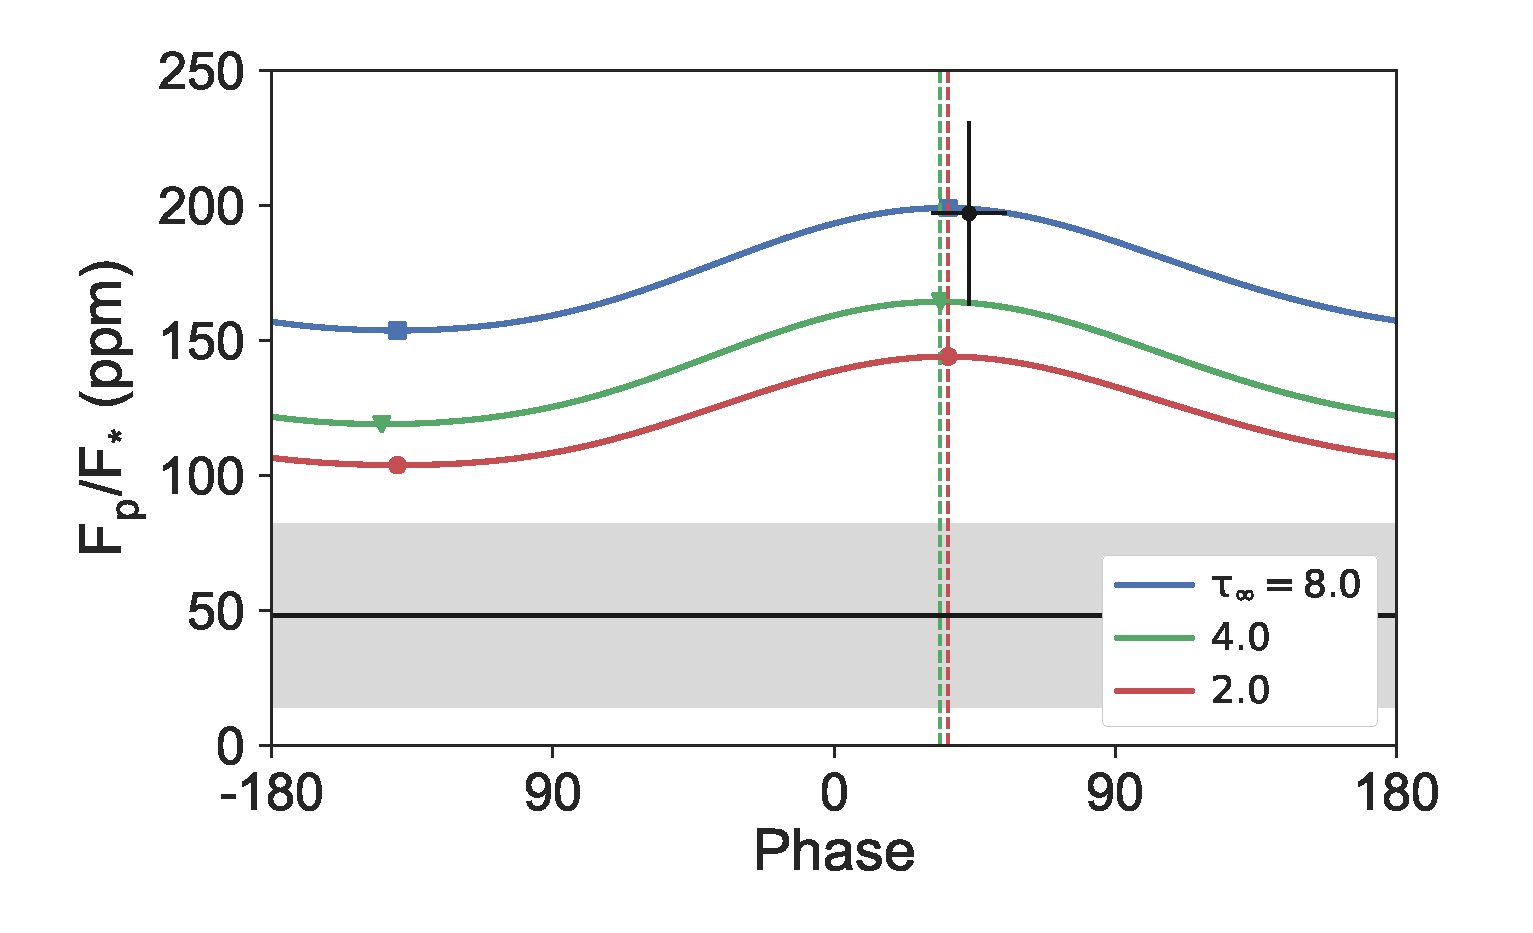
\includegraphics[width=0.75\textwidth]{figures/linking-climate-55cnce/phasecurves_vs_tau.eps}
\caption{Phase curves calculated from the emission of the half-surface-pressure level of the 5 bar \SI{4.6}{\gram\per\mole} H\textsubscript{2} + N\textsubscript{2} atmospheres (Tests 9, 10 and 11) with optical thicknesses of 2.0, 4.0, and 8.0, corresponding to the temperature maps in Figure \ref{fig:vary_tau_maps}.\label{fig:phasecurves_tauinf}}
\end{figure}

%SUBSECTION --




\subsection{Condensables and Clouds}\label{sec:condensables}


All the phase curves calculated from the simulations in this chapter had higher thermal emission from their night-side than was observed in the phase curve. This section will discuss the possibility that clouds form on the night-side, raising the radiating level and lowering the brightness temperature and night-side flux. I will post-process the simulation results to estimate where clouds could form, and will show their effect on the phase curve of the ``best-fit'' case, Test 4.

These clouds could be formed by condensables such as SiO or Na outgassed from a day-side magma ocean. \citet{miguel2011compositions} calculated the partial pressures of different species outgassed by a silicate magma in a vacuum at different temperatures. A magma ocean at \SI{2700}{\kelvin} would support significant partial pressures of various species, dominated by SiO and Na with partial pressures of about \SI{10}{\milli\bar}. For the higher surface temperatures of over \SI{3000}{\kelvin} in some tests, SiO becomes more abundant with partial pressures of hundreds of \SI{}{\milli\bar}.


\begin{figure}
\centering
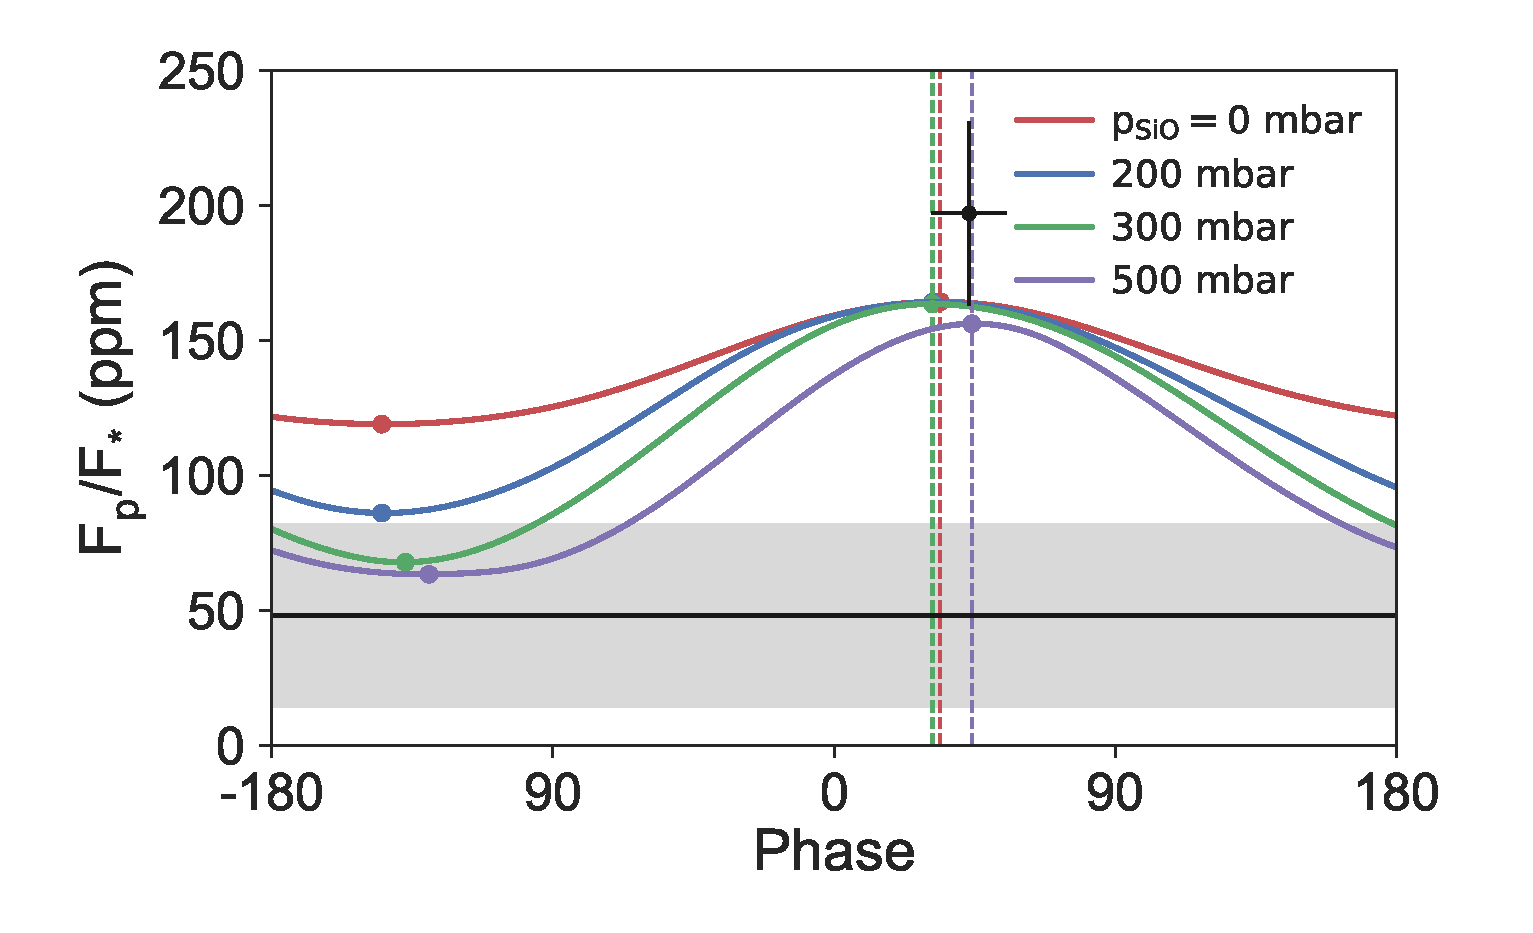
\includegraphics[width=0.75\textwidth]{figures/linking-climate-55cnce/phasecurves_clouds.eps}
\caption{Phase curves from the thermal emission of the half-surface-pressure level of Test 4, modified to estimate the effects of cloud formation from different global partial pressures of SiO. The phase curve with a partial pressure of \SI{300}{\milli\bar} of SiO shows that clouds could form on the day-side at high enough surface partial pressures.  The offset and amplitude of the \SI{300}{\milli\bar} case almost agrees with the observed phase curve within error.} \label{fig:phasecurves_clouds}
\end{figure}


I used \citet{miguel2011compositions} to calculate the partial pressures of SiO and Na based on a range of possible surface temperatures, and assumed that these were mixed uniformly with the rest of the atmosphere. I chose to test whether clouds could form at the top of the atmosphere, as this gives an upper bound on their effect on the thermal emission \citep{parmentier2016transitions}. I calculated the saturation vapour pressure of each species at the top of each column \citep{wetzel2013sio}. Estimating the effect of the clouds If the partial pressure is greater than the saturation vapour pressure, I assumed that clouds have formed in that column and set the radiating level to the top of the atmosphere.

This approximate calculation showed that SiO could condense on the night-side of some tests including Test 4, but that Na would not condense in any tests. Figure \ref{fig:phasecurves_clouds} shows that at high enough partial pressures of SiO, the clouds could significantly increase the day-night contrast and phase curve amplitude. For a partial pressure of \SI{300}{\milli\bar}, the new post-processed phase curve matches the observations of \citet{demory201655cnce} within error. Figure \ref{fig:phasecurves_clouds} also shows that cloud formation around the cool west terminator can increase the hot-spot shift, for high enough partial pressures of SiO. This is similar to the heterogenous day-side cloud formation shown to affect phase curves by  \citet{parmentier2016transitions}. This effect is small in the tests in this chapter, but could be more important for optical phase curves, as clouds can affect the atmospheric albedo very strongly.

In summary, SiO outgassed from a magma ocean is a plausible candidate for a cloud species that would form on 55 Cancri e and affect the observed phase curve. It could form high on the cooler night-side, raising the radiating level and reducing the thermal flux observed from the night-side. This could explain the difference between the modelled and observed night-side flux in the simulations. Further observations at optical wavelengths could test for the presence of clouds, which would help to explain the features of the thermal phase curve \citep{dragomir2012most}. A better understanding of the species outgassed by a magma ocean would also help to predict the possible cloud formation on 55 Cancri e \citep{miguel2011compositions}.


%SECTION CONCLUSIONS



%%%%%%%%%%%%%%%%%%%%%%%%%%%%%%%%%%%%
%SECTION  6 -- DISCUSSION
\section{Discussion}\label{sec:discussion}

The simulation results constrain the atmospheric composition and parameters of 55 Cancri e. Test 4 fitted the observations the most closely. It was a 90\%-10\% mixture of H\textsubscript{2} and N\textsubscript{2} with $\mu =$ \SI{4.6}{\gram\per\mole}, specific heat capacity \SI{7443}{\joule\per\kilogram\per\kelvin}, optical thickness 4.0, and surface pressure \SI{5}{\bar}. These are similar to the parameters predicted to fit the observations by the scaling relations of \citet{zhang2017dynamics} in Figure \ref{fig:param_map}. This test did not exactly match the observations of \citet{demory201655cnce}, but confirmed that the scaling relations are broadly accurate. This means that while the idealised model cannot exactly fit the phase curve, it can constrain the atmospheric composition. The results suggest that the atmosphere must have a mean molecular weight above \SI{2}{\gram\per\mole} and a surface pressure above 1 bar. Surface pressures of over 10 bar could be possible given a higher atmospheric molecular weight. The results also point towards the presence of night-side clouds lowering the observed brightness temperature, as have been used to explain observations of hot Jupiters \citep{parmentier2016transitions}.

The results in this chapter can be analysed using the wave-based theory in Chapter \ref{ch:wave-mean-flow}, rather than the advection-based scaling relations of \citet{zhang2017dynamics}. Tests 1 and 2 follow the qualitative predictions of the wave-based theory. Test 1 has a long radiative timescale due to its low mean molecular weight, so has a low radiative damping rate $\alpha$. This means that the wave-1 response due to the day-night forcing will be weak in comparison to the wave-0 response due to the geostrophically balanced jet -- exactly what is seen in the earlier plots of the zonally homogeneous temperature field of Test 1. In addition, the low damping rate $\alpha$ in Test 1 is dominated by the jet speed $U$ in the expression for the hot-spot shift (Equation \ref{eqn:am-U0}). This results in the large hot-spot shift in Figure \ref{fig:Tlevels-maps}.

Test 2 also behaves as expected from the wave-based theory. The short radiative timescale due to the N$_{2}$ atmosphere corresponds to a high radiative damping rate $\alpha$, giving a very strong wave-1 response. This causes the strong day-night contrast in Test 2, as this response dominates the wave-0 response from the jet. This test has no hot-spot shift, which can be explained as the high damping rate $\alpha$ dominating the jet speed $U$ in Equation \ref{eqn:am-U0}. This means that the real part of the denominator in Equation \ref{eqn:am-U0} dominates the imaginary part, and the wave response is mostly in phase with the forcing, giving a pattern similar to the response to forcing plotted in \citet{matsuno1966quasi}.

The wave-based and advection-based theories both give similar predictions for the global circulation patterns. Which theory is a better description of the global circulation of a tidally locked planet? \citet{perez2013atmospheric} use a theory based on wave transport (not stationary waves, as in Chapter \ref{ch:wave-mean-flow}) to argue that the wave timescale is key to the global circulation of hot Jupiters, not the advective timescale. This agrees with the wave-based theory in this thesis. \citet{perez2013atmospheric} suggest that the two different interpretations give similar results because the wave timescale and advective timescale are similar on hot Jupiters.

 I suggest that they reflect the same fundamental physics and have different uses. The wave-based theory matches the two-dimensional field seen in the GCM, explains the form of the hot-spot shift and night-side cyclones, and shows how the strengths of the wave response and jet height field vary relative to each other. But, the advection-based theory supplies useful predictions of real observational features such as day-night contrast and hot-spot shift, which are harder to produce from the more idealised wave-based picture. Ultimately, both pictures are useful for different situations. -- further work could use the wave-based theory to provide more practical scaling relations for real observable features.


% Tidal heating could also play a role in the temperature distribution.

% TO DO
% \subsection{Analysis using Wave-Based Theory}
%
% N2 has alpha larger than kU and omega, so response centered.
%
% H2 has omega larger than alpha and ku (U small from small alpha), so reverse hss
%
% Mixture has kU dominant (like tide-locked earth cases)


%SECTION CONCLUSIONS



%%%%%%%%%%%%%%%%%%%%%%%%%%%%%%%%%%%%
\section{Conclusions}
%CONCLUSIONS

The thermal phase curve of 55 Cancri e observed by \citet{demory201655cnce} is a puzzle. It implies a large hot-spot shift and a large day-night temperature contrast, features which should be mutually exclusive. This chapter used idealised simulations of atmospheres on 55 Cancri e to show that the phase curve can be partially matched by an atmosphere with the correct properties. The results of these simulations qualitatively matched the predictions of scaling relations for the global circulation of tidally locked planets.


The ``best-fit'' atmospheric simulation, Test 4, had a surface pressure of \SI{5}{\bar} and a mean molecular weight of \SI{4.6}{\gram\per\mole}. It matched the phase shift and maximum amplitude of the observed thermal phase curve. However, it was too warm on the night-side to match the observed night-side flux, which was a problem for all the simulations in this chapter. Using a simple estimate of where SiO clouds could form, I showed that night-side cloud formation on the night-side could raise the radiating level and lower the brightness temperature.

The simulations suggested that the observations at \SI{4.5}{\micro\metre} correspond to an absorption window. This was because they required an atmosphere with a strong greenhouse effect, that was emitting from a relatively high pressure at the observed wavelength. Further observations such as broadband phase curve or measurements at optical wavelengths could constrain the temperature of the planet better, or test for the presence of clouds. This would be very valuable to further, more realistic atmospheric modelling.

In summary, this chapter has shown that the observed thermal phase curve of 55 Cancri e can be explained by an atmosphere with a surface pressure of \SI{5}{\bar} and a mean molecular weight of \SI{4.6}{\gram\per\mole}, with a mechanism such as cloud formation to lower the night-side brightness temperature. The suite of GCM tests were consistent with the theories of atmospheric circulation discussed so far in this thesis, but could only partially match the observed phase curve. Chapter \ref{ch:clouds-lava-planets} will use a model with more detailed radiative transfer to investigate this problem further.


%RESTATE SECTION CONCLUSIONS

%OPEN OUT CONCLUSIONS

% \bibliographystyle{unsrtnat}
% \bibliography{../references.bib}
